% ============================================================================
% Text-to-Speech Architectures for Real-Time Game Dialogue
% Master's dissertation working document — full technical depth, self-contained.
% Grounded in the DeepUnity InferenceEngine project (Kokoro-82M, CosyVoice3-0.5B,
% Chatterbox-Turbo GPU ports). Compile with pdflatex.
% ============================================================================
\documentclass[11pt,a4paper]{article}

\usepackage[utf8]{inputenc}
\usepackage[T1]{fontenc}
\usepackage{lmodern}
\usepackage{microtype}
\usepackage[margin=2.5cm]{geometry}
\usepackage{amsmath,amssymb,mathtools}
\usepackage{booktabs}
\usepackage{array}
\usepackage{xcolor}
\usepackage{tikz}
\usetikzlibrary{arrows.meta,positioning,calc,fit,backgrounds,decorations.pathreplacing,shapes.geometric}
\usepackage{caption}
\usepackage{enumitem}
\usepackage[hidelinks]{hyperref}

% ---------------------------------------------------------------------------
% Palette + TikZ styles
% ---------------------------------------------------------------------------
\definecolor{cText}{HTML}{37474F}
\definecolor{cLM}{HTML}{1565C0}      % autoregressive / language model stages
\definecolor{cFlow}{HTML}{6A1B9A}    % acoustic model / flow stages
\definecolor{cVoc}{HTML}{2E7D32}     % vocoder stages
\definecolor{cCond}{HTML}{E65100}    % conditioning / style
\definecolor{cAudio}{HTML}{00695C}   % audio transport
\definecolor{cGrey}{HTML}{78909C}
\definecolor{cWarn}{HTML}{C62828}

\tikzset{
  blk/.style={draw=cGrey, thick, rounded corners=2pt, fill=white,
              minimum height=7.5mm, inner sep=4pt, font=\small, align=center},
  lmblk/.style={blk, fill=cLM!12, draw=cLM},
  flowblk/.style={blk, fill=cFlow!10, draw=cFlow},
  vocblk/.style={blk, fill=cVoc!12, draw=cVoc},
  condblk/.style={blk, fill=cCond!12, draw=cCond},
  audioblk/.style={blk, fill=cAudio!12, draw=cAudio},
  databox/.style={draw=cGrey, densely dashed, rounded corners=1pt, fill=cGrey!8,
                  inner sep=3pt, font=\scriptsize, align=center},
  arr/.style={-{Stealth[length=2.2mm]}, thick, cText},
  condarr/.style={-{Stealth[length=2mm]}, thick, cCond, densely dashed},
  lbl/.style={font=\scriptsize, text=cText},
  tick/.style={font=\tiny, text=cGrey}
}

% ---------------------------------------------------------------------------
% Notation macros (consistent across the document)
% ---------------------------------------------------------------------------
\newcommand{\RTF}{\ensuremath{\mathrm{RTF}}}
\newcommand{\TTFA}{\ensuremath{\mathrm{TTFA}}}
\newcommand{\ftok}{\ensuremath{f_{\mathrm{tok}}}}   % speech-token rate (25 Hz)
\newcommand{\fmel}{\ensuremath{f_{\mathrm{mel}}}}   % mel frame rate (50 Hz)
\newcommand{\fs}{\ensuremath{f_{s}}}                % audio sample rate (24 kHz)
\newcommand{\vth}{\ensuremath{v_\theta}}
\newcommand{\mel}{\ensuremath{\mathbf{m}}}
\newcommand{\R}{\mathbb{R}}
\newcommand{\E}{\mathbb{E}}
\newcommand{\code}[1]{\texttt{#1}}

\title{\textbf{Text-to-Speech Architectures for Real-Time Game Dialogue:}\\
\Large Autoregressive Token Synthesis, Streaming Schedules, and\\
GPU Inference Inside a Game Engine}
\author{Radu Ciobanu}
\date{July 2026 --- working draft}

\begin{document}
\maketitle

\begin{abstract}
\noindent
Large-language-model-driven non-player characters (NPCs) generate dialogue text as an
open-ended token stream; giving them a voice requires a text-to-speech (TTS) system that
converts that stream into audio \emph{while it is still being written}, on the same GPU
that renders the game, without ever stalling a frame. This document develops the problem
top-down: it defines the latency metrics that govern interactive speech
(time-to-first-audio, real-time factor, per-frame synthesis budget), builds a taxonomy of
modern neural TTS architecture families --- non-autoregressive parallel pipelines
(StyleTTS2 lineage, instantiated by Kokoro-82M), autoregressive discrete-token two-stage
systems (instantiated by CosyVoice3-0.5B), and offline-designed flow systems retrofitted
for streaming (Chatterbox-Turbo) --- and argues that the autoregressive token
architecture is the only \emph{real-time-native} design: its causal factorization admits
token-level chunked emission with bounded lookahead while preserving utterance-scale
prosody. Each family is dissected to full architectural depth, with the mathematics that
carries real design weight: conditional flow matching and its classifier-free-guided
Euler solver, finite scalar quantization, duration--alignment expansion, and
neural-source-filter vocoding. A dedicated part treats the systems side, which is the
dissertation's novel angle: running all three families entirely as HLSL compute kernels
inside the Unity game engine --- frame-budget discipline via MAC-sliced coroutines,
latent (budgeted, proximity-triggered) weight streaming, and int8 quantization analyzed
through the memory-bound/dispatch-bound lens. All quantitative claims are grounded in
measured results from the DeepUnity InferenceEngine project, validated stage-by-stage
against PyTorch reference implementations at correlation gates of $0.99$--$1.000000$.
\end{abstract}

\tableofcontents
\newpage

% ============================================================================
\section{Introduction: giving LLM-driven NPCs a real-time voice}
\label{sec:intro}
% ============================================================================

The classical production pipeline for game dialogue --- write lines, record actors, ship
static audio files --- collapses the moment an NPC's dialogue is \emph{generated} rather
than authored. A conversational NPC backed by an on-device language model produces text
that did not exist a frame earlier; there is nothing to pre-record. Speech must be
synthesized at play time, from text that arrives incrementally as the LLM decodes, on
hardware that is simultaneously busy rendering the game world. Three properties follow
immediately, and together they define the engineering problem of this document:

\begin{enumerate}[leftmargin=2em]
\item \textbf{Latency is perceptual, not throughput-statistical.} A player who asks an
NPC a question tolerates roughly the pause of human turn-taking. What matters is the time
from ``the NPC decides to speak'' to ``the first audible sample leaves the speaker''
(time-to-first-audio, \TTFA{}), and, once audio has started, that it never starves
(sustained real-time factor, \RTF{}). Total synthesis time for the whole utterance is
almost irrelevant if the first second is available early and production stays ahead of
playback.
\item \textbf{The GPU is shared and frame-locked.} Unlike a server TTS deployment, the
synthesizer does not own the device. The game renders at 30--60\,Hz; a frame that takes
longer than 33.3\,ms (at 30\,FPS) or 16.7\,ms (at 60\,FPS) is a visible hitch. Every
kernel the TTS dispatches competes with the renderer, so synthesis must be
\emph{sliceable}: decomposable into bounded pieces that interleave with rendering,
never absorbing a whole frame.
\item \textbf{The input is itself a stream.} The LLM emits text token-by-token at some
rate; the TTS must compose with that stream. The end-to-end problem is therefore
\emph{streaming text $\rightarrow$ streaming audio}: a composition of two incremental
processes with different natural granularities (subword text tokens vs.\ audio samples),
mediated by whatever intermediate representation the TTS architecture exposes. The
architecture family determines the finest granularity at which this composition can
happen --- and that granularity, more than raw model speed, determines \TTFA{} and
prosodic quality.
\end{enumerate}

This document studies the three architecture families that dominate contemporary neural
TTS through the lens of these constraints, using three concrete systems that were ported
--- weights, kernels, and streaming logic --- into the Unity game engine as part of the
DeepUnity InferenceEngine project:

\begin{itemize}[leftmargin=2em]
\item \textbf{Kokoro-82M} (StyleTTS2 lineage): a \emph{non-autoregressive parallel}
pipeline --- phonemes in, one feed-forward pass, waveform out. Extremely fast
(measured $\RTF{}=0.24$--$0.43$ on an RTX~4060) but structurally limited to
\emph{chunk-level} streaming: nothing can be emitted before a whole text chunk is
synthesized (Section~\ref{sec:kokoro}).
\item \textbf{CosyVoice3-0.5B}: an \emph{autoregressive discrete-token two-stage} system
--- a text LLM emits 25\,Hz speech tokens which a chunk-aware causal flow-matching model
renders to mel and a causal vocoder to waveform. Streaming-native: audio can be emitted
every 25 generated tokens with 3 tokens of lookahead, and earlier audio never changes
(Section~\ref{sec:cosy}).
\item \textbf{Chatterbox-Turbo}: an AR token model paired with a \emph{bidirectional}
flow decoder designed for offline use --- the instructive contrast case. Its acoustic
model needs the whole token sequence at once, so streaming had to be retrofitted at
clause granularity, and window-level retrofits hit measurable seam artifacts
(Section~\ref{sec:chatterbox}).
\end{itemize}

The central technical claim, developed in Sections~\ref{sec:cosy}
and~\ref{sec:streaming}, is that the AR discrete-token architecture is
\emph{real-time-native}: causality is present at every stage of its pipeline (AR language
model, chunk-causal attention in the flow, causal convolutions in the vocoder), so the
system can commit to a prefix of the utterance and extend it indefinitely --- exactly the
contract a streaming audio ring buffer requires --- while conditioning every new chunk on
the full acoustic history, which preserves utterance-scale prosody. Non-AR systems, by
contrast, realize global utterance statistics (durations, instance-normalization moments)
up front, which makes them \emph{fast} but forces prosody to reset at every chunk
boundary.

The second half of the document (Sections~\ref{sec:engine}--\ref{sec:results}) treats
what is, to the author's knowledge, the least-documented part of the problem and the
dissertation's novel contribution: running these models \emph{inside} a game engine with
no ML runtime at all --- every stage hand-written as HLSL compute kernels, weights
streamed onto the GPU under per-frame byte budgets tied to player proximity, synthesis
sliced by a MAC-accounting coroutine so that a speaking NPC costs 2 dropped frames in
5544, and quantization decisions made by profiling whether a stage is memory-bound or
dispatch-bound rather than by assumption.

\paragraph{Provenance of numbers.} Every measured figure in this document comes from the
DeepUnity InferenceEngine project logs (RTX~4060 laptop GPU unless stated otherwise), and
every ported model was validated stage-by-stage against its PyTorch reference via a
parity harness (per-stage \code{.npy} dumps, fixed seeds, noise exported as tensors;
Section~\ref{sec:parity}) with per-stage correlation gates that the shipped ports pass at
$0.999$--$1.000000$. Architectural constants are quoted from the frozen port
specifications, which were themselves verified against checkpoint tensor shapes at
export time.

% ============================================================================
\section{The real-time contract: metrics and budgets}
\label{sec:metrics}
% ============================================================================

\subsection{Real-time factor and time-to-first-audio}
\label{sec:rtf}

Let an utterance synthesize in wall-clock time $T_{\mathrm{wall}}$ and produce audio of
duration $T_{\mathrm{audio}}$. The \emph{real-time factor} is
\begin{equation}
\RTF \;=\; \frac{T_{\mathrm{wall}}}{T_{\mathrm{audio}}},
\label{eq:rtf}
\end{equation}
with the convention used throughout this document that $\RTF < 1$ means
faster-than-real-time (some literature uses the reciprocal; we do not). For \emph{offline}
synthesis, \RTF{} is the whole story. For \emph{streaming} synthesis two refinements are
needed. First, the metric that dominates perceived responsiveness is the
\emph{time-to-first-audio},
\begin{equation}
\TTFA \;=\; t_{\mathrm{first\ sample\ audible}} - t_{\mathrm{synthesis\ requested}},
\label{eq:ttfa}
\end{equation}
which decomposes along the pipeline's critical path. For a chunked AR system that must
accumulate $N_1$ tokens before the first acoustic chunk can be rendered
(Section~\ref{sec:schedule}),
\begin{equation}
\TTFA \;=\;
\underbrace{T_{\mathrm{prefill}}}_{\text{prompt}+\text{text}}
+ \underbrace{\frac{N_1}{r_{\mathrm{LM}}}}_{\text{token decode}}
+ \underbrace{T_{\mathrm{flow}}(C_1)}_{\text{first chunk ODE}}
+ \underbrace{T_{\mathrm{voc}}(C_1)}_{\text{first chunk vocode}}
+ \underbrace{T_{\mathrm{xfer}} + T_{\mathrm{prebuf}}}_{\text{readback, ring prebuffer}},
\label{eq:ttfa-decomp}
\end{equation}
where $r_{\mathrm{LM}}$ is the LM decode rate in tokens/s and $C_1$ the first chunk's
frame extent. Second, sustained playback without starvation requires the
\emph{steady-state} production rate to meet consumption:
\begin{equation}
\text{for every chunk } k:\qquad
\sum_{j \le k} T_{\mathrm{synth}}(j) \;\le\; \TTFA + \sum_{j < k} T_{\mathrm{audio}}(j),
\label{eq:no-starve}
\end{equation}
i.e.\ cumulative synthesis time must never overtake cumulative audio released plus the
initial head start. A system can have $\RTF > 1$ overall yet stream acceptably for short
utterances if \TTFA{} is small and the ring buffer is deep --- but only $\RTF \le 1$
(with margin for frame-slicing overhead, Section~\ref{sec:framebudget}) guarantees
starvation-free playback of arbitrary-length utterances. For the AR token systems studied
here there is an additional \emph{per-stage} real-time condition with a clean closed
form: a 25\,Hz token LM feeding a streaming pipeline must decode at
$r_{\mathrm{LM}} \ge \ftok = 25$\,tokens/s, or the acoustic stages will drain the token
queue no matter how fast they are. (The DeepUnity CosyVoice3 LM measures
49.8\,tokens/s on the RTX~4060 --- $2.0\times$ the real-time token rate --- so the LM is
not the binding constraint there; the flow is. Section~\ref{sec:results}.)

\subsection{The frame-time budget on one shared GPU}
\label{sec:framebudget}

A game targeting 30\,FPS has a 33.3\,ms frame; at 60\,FPS, 16.7\,ms. Rendering,
simulation, and \emph{every other} neural system (the dialogue LLM itself, speech
recognition for the player's microphone) share it. The synthesis budget is therefore not
``the GPU'' but a \emph{slice} of each frame --- empirically 2--3\,ms of GPU work per
frame is invisible next to a 30\,FPS render load, and this is exactly how the DeepUnity
runtime sizes its slices (a MAC-accounting budget of $2.5\times 10^{8}$
multiply-accumulates per yield on the RTX~4060; Section~\ref{sec:slicing}).

Two consequences deserve emphasis because they shape everything downstream. First,
\emph{effective} \RTF{} inside a game is worse than benchtop \RTF{}: if synthesis may
only occupy a fraction $\beta$ of each frame, wall-clock synthesis time inflates by
$\approx 1/\beta$, so a model with benchtop $\RTF = 0.3$ at $\beta = 0.15$ is only just
real-time in-engine. Any architecture whose benchtop \RTF{} is near 1 is \emph{not}
viable on that hardware tier, no matter how it streams. Second, latency spikes are worse
than average load: a single 200\,ms flow-matching solve dispatched monolithically is a
6-frame freeze even though its \emph{average} cost amortized over a second is trivial.
Real-time TTS in-engine is thus as much a \emph{scheduling} problem as a model-speed
problem, which is why Section~\ref{sec:engine} treats the slicing machinery as a
first-class architectural component.

\subsection{Streaming text $\rightarrow$ streaming audio: the composition problem}
\label{sec:composition}

The dialogue LLM produces a text-token stream at its own decode rate; the player hears an
audio-sample stream at exactly $\fs = 24\,000$ samples/s. Between them sits the TTS,
and the composition has to be analyzed as a pipeline of \emph{commit points}: positions
in the stream where a stage has enough input to produce output that will never be
retracted. Each architecture family exposes different commit points:

\begin{itemize}[leftmargin=2em]
\item \textbf{Text side.} Subword tokens are not a valid TTS input granularity --- a
grapheme-to-phoneme frontend or a text LM needs at least lexically complete words, and
prosody models want clause- or sentence-level context (a question mark at the end of a
sentence changes the pitch contour of its beginning). The practical commit point for
feeding TTS is the \emph{clause}: the DeepUnity \code{KokoroVoice.FeedText} interface
accumulates LLM text deltas and cuts only at sentence enders (\code{. ! ? ;} and
newline), with a comma-cut escape hatch after 220 pending characters for run-on
sentences. The same interface drives CosyVoice3, whose (non-bistream) LM conditions on
the complete utterance text before decoding speech tokens --- so text enters both systems
at clause granularity, and the interesting differences are all downstream.
\item \textbf{Acoustic side.} This is where the families diverge. A non-AR model's
commit point is the whole clause (one parallel forward realizes all of it, and internal
whole-chunk statistics mean no prefix is final until the pass completes,
Section~\ref{sec:kokoro-noar}). An AR token model's commit point is the \emph{token
chunk}: 25 tokens ($=1$\,s of audio) plus 3 tokens of lookahead suffice to render audio
that is bit-exact with what an offline render of the full utterance would have produced
in that interval (Section~\ref{sec:schedule}). An offline-designed flow model has no
commit point short of the full clause, and attempts to impose one by windowing leave
measurable seams (Section~\ref{sec:chatterbox-stream}).
\item \textbf{Transport side.} All three ports converge on the same audio transport: a
lock-protected ring buffer filled by the synthesis coroutine on the main thread and
drained by the audio thread's PCM callback, with a prebuffer threshold (0.4\,s in
\code{KokoroVoice}) trading first-sound latency against underrun robustness, and a
monotonic written/read sample counter pair that also drives audio-synchronized subtitle
reveal (Section~\ref{sec:sync-ux}).
\end{itemize}

The pipeline's \TTFA{} is governed by its \emph{coarsest} early commit point. This is
the precise sense in which architecture choice is a latency decision before it is a
quality decision, and it is why the taxonomy of the next section is organized around
causality structure rather than around acoustic modeling technique.

% ============================================================================
\section{A taxonomy of neural TTS architecture families}
\label{sec:taxonomy}
% ============================================================================

Modern neural TTS pipelines factor the map
$\text{text} \rightarrow \text{waveform}$ through intermediate representations, and the
useful classification axis for real-time work is \emph{where autoregression (temporal
causality) lives}, because that determines the streaming commit points of
Section~\ref{sec:composition}. Three families cover the systems that matter in 2026:

\begin{description}[leftmargin=2em, style=nextline]
\item[Family A --- Non-autoregressive parallel pipelines.] Descendants of
FastSpeech~2 and StyleTTS~2: an explicit \emph{duration model} replaces autoregressive
alignment; text-rate features are expanded to frame rate by a predicted hard alignment;
prosody (F0, energy) is regressed in parallel; a GAN-trained vocoder head emits the
waveform. One feed-forward pass per text chunk, no sampling loop, no KV cache. Exemplar:
\textbf{Kokoro-82M} (Section~\ref{sec:kokoro}).
\item[Family B --- Autoregressive discrete-token two-stage systems.] Descendants of the
neural-codec-LM line (VALL-E, Tortoise, and the CosyVoice series): a speech tokenizer
defines a low-rate discrete code (here 25\,Hz finite-scalar-quantized tokens); a text LM
autoregressively generates those tokens; a separately trained acoustic decoder
(here a conditional flow-matching diffusion transformer) renders token chunks to mel; a
causal vocoder renders mel to waveform. Causality at every stage. Exemplar:
\textbf{CosyVoice3-0.5B} (Section~\ref{sec:cosy}).
\item[Family C --- AR front-end with offline acoustic decoder.] Hybrids that generate
tokens autoregressively but decode them with a \emph{bidirectional} acoustic model that
attends over the whole utterance --- a design optimal for offline quality benchmarks and
structurally hostile to streaming. Exemplar: \textbf{Chatterbox-Turbo}
(Section~\ref{sec:chatterbox}).
\end{description}

Figure~\ref{fig:taxonomy} shows the three families side by side with their streaming
commit points marked; Table~\ref{tab:families} summarizes the comparison, including the
measured end-to-end numbers from the DeepUnity ports that later sections unpack.

\begin{figure}[htbp]
\centering
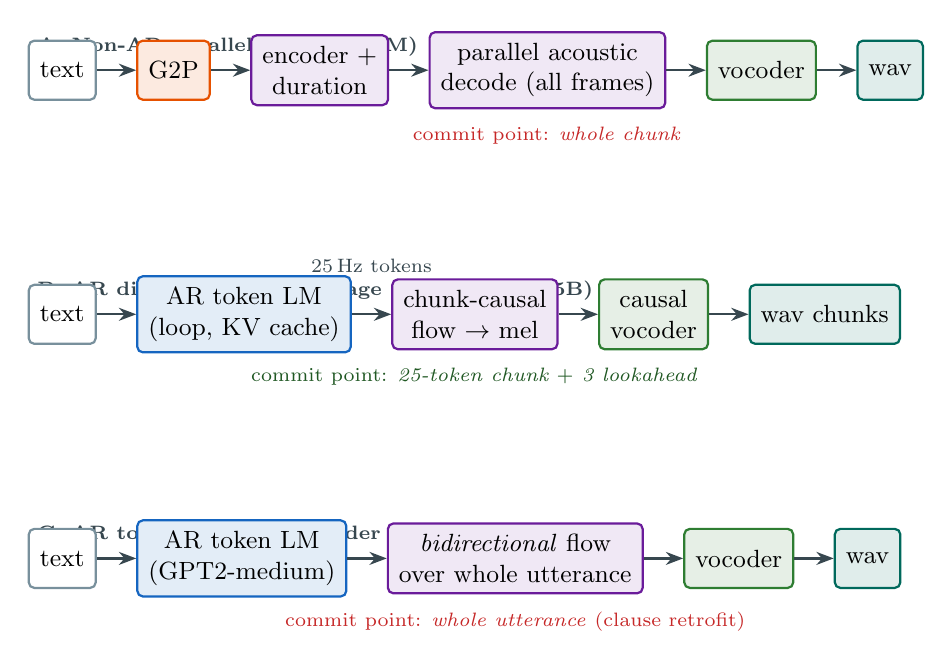
\begin{tikzpicture}[node distance=4mm and 5mm]
% ----- Family A lane -----
\node[lbl, anchor=west] (la) at (0,0) {\textbf{A. Non-AR parallel (Kokoro-82M)}};
\node[blk, below=3mm of la.west, anchor=west] (a1) {text};
\node[condblk, right=of a1] (a2) {G2P};
\node[flowblk, right=of a2] (a3) {encoder $+$\\duration};
\node[flowblk, right=of a3] (a4) {parallel acoustic\\decode (all frames)};
\node[vocblk, right=of a4] (a5) {vocoder};
\node[audioblk, right=of a5] (a6) {wav};
\draw[arr] (a1) -- (a2); \draw[arr] (a2) -- (a3); \draw[arr] (a3) -- (a4);
\draw[arr] (a4) -- (a5); \draw[arr] (a5) -- (a6);
\node[lbl, text=cWarn, below=1mm of a4] {commit point: \emph{whole chunk}};
% ----- Family B lane -----
\node[lbl, anchor=west] (lb) at (0,-3.1) {\textbf{B. AR discrete-token two-stage (CosyVoice3-0.5B)}};
\node[blk, below=3mm of lb.west, anchor=west] (b1) {text};
\node[lmblk, right=of b1] (b2) {AR token LM\\(loop, KV cache)};
\node[flowblk, right=of b2] (b3) {chunk-causal\\flow $\to$ mel};
\node[vocblk, right=of b3] (b4) {causal\\vocoder};
\node[audioblk, right=of b4] (b5) {wav chunks};
\draw[arr] (b1) -- (b2);
\draw[arr] (b2) -- (b3) node[midway, above=4mm, lbl] {25\,Hz tokens};
\draw[arr] (b3) -- (b4); \draw[arr] (b4) -- (b5);
\node[lbl, text=cVoc!70!black, below=1mm of b3] {commit point: \emph{25-token chunk $+$ 3 lookahead}};
% ----- Family C lane -----
\node[lbl, anchor=west] (lc) at (0,-6.2) {\textbf{C. AR tokens $+$ offline decoder (Chatterbox-Turbo)}};
\node[blk, below=3mm of lc.west, anchor=west] (c1) {text};
\node[lmblk, right=of c1] (c2) {AR token LM\\(GPT2-medium)};
\node[flowblk, right=of c2] (c3) {\emph{bidirectional} flow\\over whole utterance};
\node[vocblk, right=of c3] (c4) {vocoder};
\node[audioblk, right=of c4] (c5) {wav};
\draw[arr] (c1) -- (c2); \draw[arr] (c2) -- (c3); \draw[arr] (c3) -- (c4);
\draw[arr] (c4) -- (c5);
\node[lbl, text=cWarn, below=1mm of c3] {commit point: \emph{whole utterance} (clause retrofit)};
\end{tikzpicture}
\caption{The three TTS architecture families, drawn as streaming pipelines with their
finest safe \emph{commit points} (positions after which emitted audio never changes)
marked. Family~B is the only one whose commit point is finer than the text chunk fed in;
that property --- not raw model speed --- is what makes it real-time-native.}
\label{fig:taxonomy}
\end{figure}

\begin{table}[htbp]
\centering
\caption{Architecture families compared. Measured values from the DeepUnity GPU ports on
an RTX~4060 laptop GPU; $\RTF < 1$ is faster than real time
(Eq.~\ref{eq:rtf}). ``Prosody scope'' = the span over which the model can plan a coherent
prosodic arc without a reset.}
\label{tab:families}
\small
\begin{tabular}{@{}p{3.4cm}p{3.6cm}p{3.8cm}p{3.6cm}@{}}
\toprule
 & \textbf{A: Non-AR parallel} & \textbf{B: AR token two-stage} & \textbf{C: AR $+$ offline decoder} \\
 & Kokoro-82M & CosyVoice3-0.5B & Chatterbox-Turbo \\
\midrule
Parameters & 82\,M & $\approx$0.5\,B LM $+$ flow/voc & $\approx$0.35\,B T3 $+$ S3Gen \\
Intermediate repr. & phoneme feats $+$ durations & 25\,Hz FSQ tokens & 25\,Hz speech tokens \\
Acoustic decode & one parallel pass & 10-step causal CFM (DiT) & 2-step bidirectional flow \\
Vocoder & ISTFTNet (NSF$+$iSTFT) & CausalHiFT (NSF$+$iSTFT) & HiFT (NSF$+$iSTFT) \\
Streaming granularity & clause (chunk-level only) & 25 tokens $=$ 1\,s ($+$3 lookahead) & clause (retrofit) \\
Prefix stability & n/a (chunk atomic) & bit-identical prefixes & re-render diverges \\
Prosody scope & one clause; resets between & full utterance (AR history) & full utterance \\
Voice cloning & fixed voicepacks (blendable) & zero-shot (prompt tokens $+$ mel $+$ x-vector) & baked reference dict \\
Stochasticity & vocoder noise only & RAS-sampled tokens $+$ fixed flow noise & sampled tokens $+$ flow \\
Measured \RTF{} @4060 & \textbf{0.24--0.43} & 2.0 offline / 2.86 streaming & 1.42 \\
Measured \TTFA{} & first-clause synth time & 4.65\,s (pre-optimization) & first-clause synth time \\
Hardware tier & low-end viable & needs optimization headroom & offline / cutscene \\
\bottomrule
\end{tabular}
\end{table}

Three orientation remarks before the deep dives. First, all three families converge on
the \emph{same vocoder science} --- a neural source-filter harmonic model driving an
iSTFT head (Section~\ref{sec:nsf}) --- so the vocoder is essentially a solved,
family-independent component; the families differ in everything upstream of mel.
Second, the families are not quality-ordered: Kokoro's fixed-voicepack, deterministic
design is a feature for a shipped game (reproducible lines, no sampling failure modes),
while CosyVoice3's zero-shot cloning and sampled prosody buy expressiveness at the price
of a sampling loop that can, rarely, misbehave and must be guarded (length caps,
Section~\ref{sec:ras}). Third, the measured \RTF{} column shows why this document spends
its systems sections on optimization: the streaming-native architecture is currently the
\emph{slowest} of the three on mid-range hardware, and closing that gap (a concrete,
profiled roadmap exists; Section~\ref{sec:roadmap}) is exactly the engineering price of
real-time-native streaming.

% ============================================================================
\section{Family A in depth: Kokoro-82M, a non-autoregressive parallel pipeline}
\label{sec:kokoro}
% ============================================================================

Kokoro-82M is a distilled member of the StyleTTS~2 lineage: a single feed-forward pass
maps a phoneme string ($\le$510 symbols) plus a 256-dimensional \emph{style vector} to a
24\,kHz waveform. There is no KV cache and no sampling loop; the only stochastic
component is the vocoder's neural-source-filter noise. At 82\,M parameters (327\,MB
fp32 checkpoint, $\approx$164\,MB fp16 export, 143\,MB int8) it is small enough for
low-end GPUs, and its measured $\RTF = 0.24$--$0.43$ on the RTX~4060 makes it the
workhorse tier of the DeepUnity NPC stack. Figure~\ref{fig:kokoro} shows the exact
inference graph; this section walks it stage by stage, because the architectural details
are precisely what create --- and what bound --- its streaming behavior.

\begin{figure}[htbp]
\centering
\resizebox{\textwidth}{!}{%
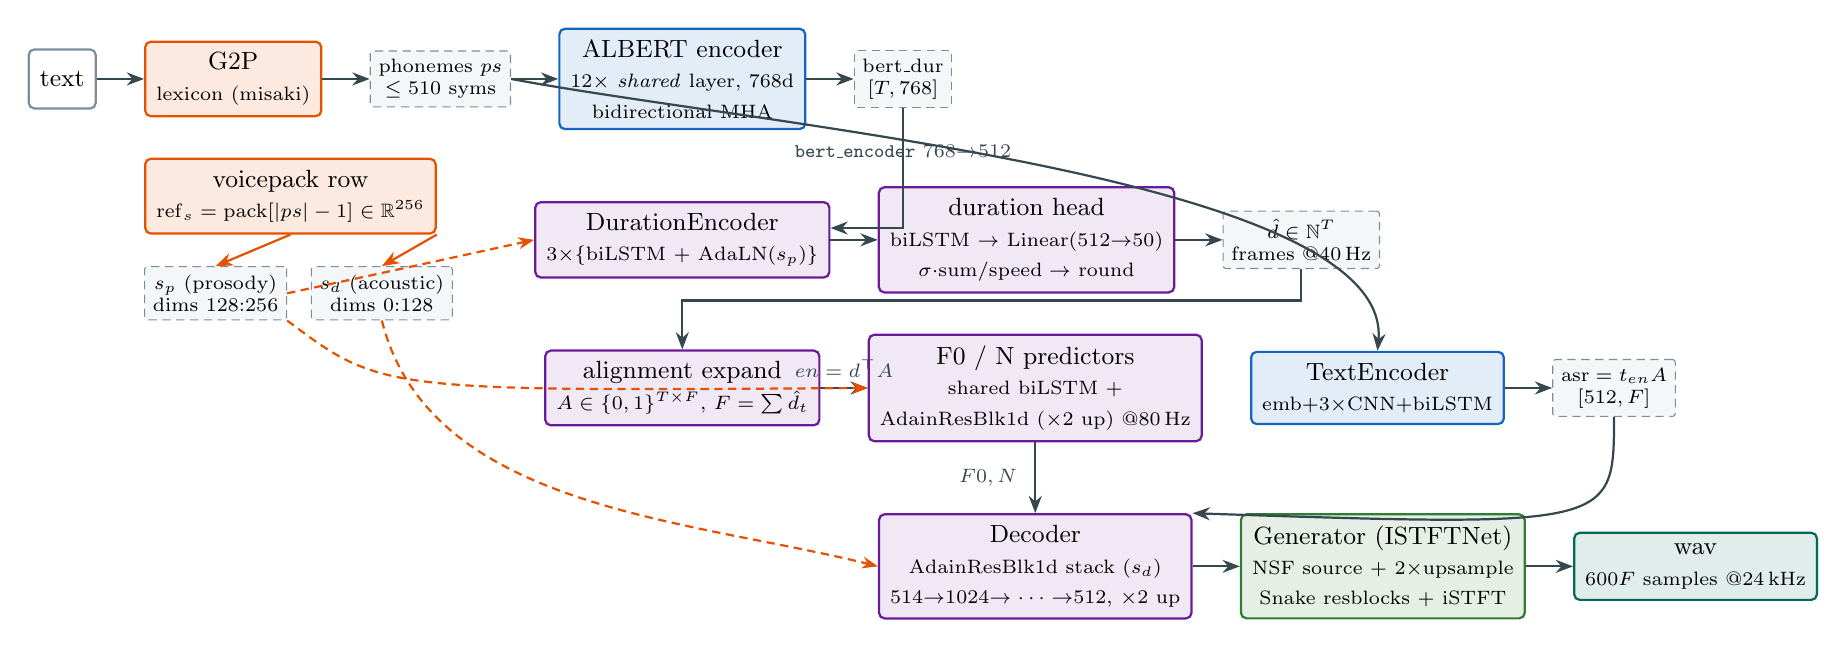
\begin{tikzpicture}[node distance=3.5mm and 6mm, font=\small]
% Row 1: frontend
\node[blk] (text) {text};
\node[condblk, right=of text] (g2p) {G2P\\\scriptsize lexicon (misaki)};
\node[databox, right=of g2p] (ps) {phonemes $ps$\\\scriptsize $\le 510$ syms};
\node[lmblk, right=of ps] (albert) {ALBERT encoder\\\scriptsize 12$\times$ \emph{shared} layer, 768d\\\scriptsize bidirectional MHA};
\node[databox, right=of albert] (bd) {$\mathrm{bert\_dur}$\\\scriptsize $[T,768]$};
\draw[arr] (text) -- (g2p); \draw[arr] (g2p) -- (ps); \draw[arr] (ps) -- (albert);
\draw[arr] (albert) -- (bd);
% Style vector (left column, below the frontend)
\node[condblk, below=10mm of g2p.west, anchor=north west] (voice) {voicepack row\\\scriptsize $\mathrm{ref}_s=\mathrm{pack}[|ps|-1]\in\R^{256}$};
\node[databox, below=4mm of voice.south west, anchor=north west] (sp) {$s_p$ (prosody)\\\scriptsize dims 128:256};
\node[databox, right=3mm of sp] (sd) {$s_d$ (acoustic)\\\scriptsize dims 0:128};
\draw[arr, cCond] (voice.south) -- (sp.north);
\draw[arr, cCond] (voice.south east) -- (sd.north);
% Row 2: prosody predictor
\node[flowblk, below=9mm of albert] (durenc) {DurationEncoder\\\scriptsize 3$\times$\{biLSTM $+$ AdaLN($s_p$)\}};
\node[flowblk, right=of durenc] (durhead) {duration head\\\scriptsize biLSTM $\to$ Linear(512$\to$50)\\\scriptsize $\sigma{\cdot}\mathrm{sum}/\mathrm{speed}\to$ round};
\node[databox, right=of durhead] (dur) {$\hat d\in\mathbb{N}^{T}$\\\scriptsize frames @40\,Hz};
\draw[arr] (bd.south) |- ($(durenc.east)+(0,1.5mm)$) node[pos=0.25, above, lbl]{\code{bert\_encoder} 768$\to$512};
\draw[arr] (durenc) -- (durhead); \draw[arr] (durhead) -- (dur);
\draw[condarr] (sp.east) .. controls +(1.4,0.3) .. (durenc.west);
% Row 3: alignment + F0/N
\node[flowblk, below=9mm of durenc] (align) {alignment expand\\\scriptsize $A\in\{0,1\}^{T\times F}$, $F=\sum \hat d_t$};
\node[flowblk, right=of align] (f0n) {F0 / N predictors\\\scriptsize shared biLSTM $+$\\\scriptsize AdainResBlk1d ($\times2$ up) @80\,Hz};
\node[lmblk, right=of f0n] (tenc) {TextEncoder\\\scriptsize emb$+$3$\times$CNN$+$biLSTM};
\node[databox, right=of tenc] (asr) {$\mathrm{asr}=t_{en}A$\\\scriptsize $[512,F]$};
\draw[arr] (dur.south) -- ++(0,-4mm) -| (align.north);
\draw[arr] (align) -- (f0n) node[midway, above, lbl]{$en = d^{\top}A$};
\draw[arr] (ps.east) .. controls +(3.2,-0.6) and +(0.2,2.2) .. (tenc.north);
\draw[arr] (tenc) -- (asr);
\draw[condarr] (sp.south east) .. controls +(1.2,-0.9) .. (f0n.west);
% Row 4: decoder + generator
\node[flowblk, below=9mm of f0n] (dec) {Decoder\\\scriptsize AdainResBlk1d stack ($s_d$)\\\scriptsize 514$\to$1024$\to\cdots\to$512, $\times2$ up};
\node[vocblk, right=of dec] (gen) {Generator (ISTFTNet)\\\scriptsize NSF source $+$ 2$\times$upsample\\\scriptsize Snake resblocks $+$ iSTFT};
\node[audioblk, right=of gen] (wav) {wav\\\scriptsize $600F$ samples @24\,kHz};
\draw[arr] (f0n) -- (dec) node[midway, left=1mm, lbl]{$F0,N$};
\draw[arr] (asr.south) .. controls +(0,-1.4) .. (dec.north east);
\draw[arr] (dec) -- (gen); \draw[arr] (gen) -- (wav);
\draw[condarr] (sd.south) .. controls +(0.6,-2.4) and +(-2.4,0.6) .. (dec.west);
\end{tikzpicture}%
}
\caption{Kokoro-82M inference graph (exact, from the port spec). One feed-forward pass
per text chunk: phonemes are encoded bidirectionally, durations are predicted and
\emph{realized immediately} as a hard alignment $A$, prosody (F0, energy $N$) is
regressed in parallel at 80\,Hz, and an AdaIN-styled decoder plus NSF-iSTFT generator
emit the waveform. Orange dashed arrows: style conditioning ($s_p$ prosody half, $s_d$
acoustic half of the 256-d voicepack row; $s_d$ also styles the generator's resblocks).
One duration frame $=$ 600 samples $=$ 25\,ms.}
\label{fig:kokoro}
\end{figure}

\subsection{Text frontend: G2P and the phoneme vocabulary}
\label{sec:kokoro-g2p}

Kokoro consumes phonemes, not graphemes: a grapheme-to-phoneme (G2P) frontend maps text
to an IPA-based symbol string $ps$, which a fixed 178-entry vocabulary maps to integer
ids (114 symbols actually used; unknown symbols are \emph{silently dropped}, a
port-critical detail since it shifts alignment lengths). The DeepUnity port uses a
dictionary-lookup G2P (gold/silver lexicon TSVs) rather than the reference's
espeak-backed fallback --- a licensing decision as much as a technical one (espeak is
GPL; the engine's asset policy is Apache/MIT/CC only). Input ids are wrapped in boundary
tokens: $\mathrm{ids} = [0, \mathrm{vocab}(ps), 0]$, and the sequence must satisfy
$T \le 512$, the ALBERT positional table size --- this hard cap is one of the two reasons
text must be chunked at clause granularity (the other is prosodic,
Section~\ref{sec:kokoro-noar}). American English G2P additionally post-maps the flap
and the glottal stop to their lexicon-internal symbols, matching reference behavior.

A subtle but consequential frontend rule: the \emph{voicepack row is selected by phoneme
string length}, $\mathrm{ref}_s = \mathrm{pack}[\,|ps|-1\,] \in \R^{1\times 256}$, from a
$[510,1,256]$ per-voice tensor --- the style vector is length-conditioned, so short and
long utterances literally use different style embeddings. Voice blending is a plain mean
of packs (the shipped \code{velmire\_elder} NPC voice is such a blend, baked from 12
packs), which works because the style space is smooth; the blend is averaged at staging
time and re-imported as a first-class voice, not blended at runtime.

\subsection{ALBERT phoneme encoder}
\label{sec:kokoro-albert}

The linguistic encoder is a phoneme-level ALBERT (``PL-BERT''): 12 transformer layers
with \emph{one shared weight set} applied twelve times --- an export-size gift (one
layer's tensors serve all twelve applications) and a scheduling gift (the GPU kernel loop
reuses one bound weight set). Embeddings are 128-d (word $+$ absolute position $+$ token
type), layer-normed, then linearly mapped $128 \to 768$; each layer is post-LN
multi-head attention (12 heads $\times$ 64) with \emph{bidirectional} (unmasked) scores,
followed by a 2048-d GELU (tanh approximation) FFN. Bidirectionality matters
architecturally: every output position sees the whole clause, so even the text encoding
is non-causal --- streaming cannot begin upstream of the acoustic model either. The
output $\mathrm{bert\_dur} \in \R^{T\times 768}$ is projected to 512 channels
(\code{bert\_encoder}) for the prosody branch.

\subsection{Duration prediction and alignment expansion}
\label{sec:kokoro-duration}

The prosody predictor concatenates the 512-d text features with the broadcast prosody
style $s_p$ (128-d) and runs a \code{DurationEncoder} of three
$\{\text{biLSTM} \to \text{AdaLN}(s_p)\}$ blocks (output re-concatenated with style each
time, giving 640 channels), then a final biLSTM and the duration head. The head is worth
writing out exactly, because it embodies the family's defining commitment. With
$h_t \in \R^{512}$ the head input at phoneme $t$ and $W \in \R^{50\times512}$:
\begin{equation}
\hat d_t \;=\; \max\!\left(1,\ \operatorname{round}\!\Big( \frac{1}{\mathrm{speed}}
\sum_{k=1}^{50} \sigma\!\big( (W h_t + b)_k \big) \Big) \right)
\qquad \in \{1,2,\dots\},
\label{eq:duration}
\end{equation}
i.e.\ 50 sigmoid ``sub-duration'' channels are \emph{summed} (not softmax-selected) and
rounded --- a soft-binned regression of each phoneme's duration in 40\,Hz frames
(1 frame $=$ 25\,ms $=$ 600 samples at 24\,kHz). The \code{speed} control divides before
rounding, giving smooth global tempo control. The total frame count
$F = \sum_t \hat d_t$ is then \emph{realized immediately} as a hard monotone alignment
matrix $A \in \{0,1\}^{T\times F}$,
\begin{equation}
A_{t,f} = 1 \iff c_{t-1} \le f < c_t, \qquad c_t = \textstyle\sum_{u\le t}\hat d_u ,
\label{eq:alignment}
\end{equation}
and every downstream tensor is produced by expanding text-rate features to frame rate
through $A$: the prosody branch consumes $en = d^{\top}A \in \R^{640\times F}$ and the
acoustic branch consumes $\mathrm{asr} = t_{en}A \in \R^{512\times F}$, where $t_{en}$
comes from a separate three-layer CNN$+$biLSTM \code{TextEncoder} over the same phoneme
ids. Equations~\eqref{eq:duration}--\eqref{eq:alignment} are the mathematical signature
of Family~A: \emph{time is allocated before any audio exists}. The utterance's temporal
skeleton --- how long every phoneme lasts, hence where every word lands --- is fixed in a
single parallel decision. This is what buys one-pass speed, and what forfeits the ability
to revise pacing as an utterance unfolds.

\subsection{F0/energy prediction and AdaIN style conditioning}
\label{sec:kokoro-f0}

Pitch and energy are regressed from the expanded features by twin convolutional stacks
(three \code{AdainResBlk1d} blocks each, the middle one upsampling $\times 2$, so F0 and
$N$ live at 80\,Hz $= 2F$ frames) after a shared biLSTM. Style enters through
\emph{adaptive instance normalization}: with per-channel, per-utterance temporal moments
$\mu_c(x), \sigma_c(x)$ computed over the frame axis,
\begin{equation}
\mathrm{AdaIN}(x, s) \;=\; \big(1+\gamma(s)\big)\odot
\frac{x - \mu_c(x)}{\sqrt{\sigma_c^2(x) + \varepsilon}} \;+\; \beta(s),
\qquad [\gamma(s);\beta(s)] = W_s s ,
\label{eq:adain}
\end{equation}
where $s$ is the relevant style half and the $(1+\gamma)$ convention (identity at
$\gamma = 0$) is a recurring normalization trap shared with, e.g., Gemma's RMSNorm.
The analogous \code{AdaLayerNorm} in the duration encoder applies the same
$(1+\gamma)\cdot\mathrm{LN}(x)+\beta$ pattern over channels. Equation~\eqref{eq:adain} is
the second family-defining formula: the normalization statistics are \emph{whole-chunk
temporal statistics}. Every styled activation depends on every frame of the chunk,
including future ones --- the network is non-causal not just in attention but in its very
normalization layers. Section~\ref{sec:kokoro-noar} draws out the streaming consequence.

The decoder proper stacks \code{AdainResBlk1d} blocks styled by the acoustic half $s_d$:
input $[\mathrm{asr}; F0; N] \in \R^{514\times F}$ (F0/N strided back to 40\,Hz by
learned $k{=}3,s{=}2$ convolutions --- the 80\,Hz$\to$40\,Hz$\to$80\,Hz round trip has
trained weights and must not be ``optimized away''), width $514\to1024\to\cdots$, with
$\mathrm{asr}$/F0/N re-concatenated at each of three blocks, and a final upsampling block
to $[512, 2F]$. Residual branches use weight-normalized $k{=}3$ convolutions with
pre-activation LeakyReLU(0.2); upsampling blocks pair a depthwise transposed-conv
$\times2$ in the residual path with nearest-neighbor $\times2$ in the shortcut, summed
with gain $1/\sqrt2$.

\subsection{Generator: NSF harmonic source plus iSTFT head}
\label{sec:kokoro-gen}

The waveform head is an ISTFTNet-style HiFiGAN variant, AdaIN-conditioned throughout,
with two upsampling stages ($\times10$, $\times6$; kernels 20, 12) and per-stage triples
of dilated \code{AdaINResBlock1}s (kernels 3/7/11, dilations 1/3/5) whose activation is
the \emph{Snake} periodic nonlinearity $x \mapsto x + \alpha^{-1}\sin^2(\alpha x)$ with a
learned per-channel $\alpha$ --- a periodicity-friendly activation that materially
improves harmonic reconstruction over LeakyReLU in GAN vocoders. Instead of upsampling
all the way to 24\,kHz, the trunk stops at $\fs/\mathrm{hop}$ with $\mathrm{hop}=5$,
$n_{\mathrm{fft}}=20$, and a final projection emits 22 channels
interpreted as 11 log-magnitudes and 11 phase angles:
\begin{equation}
\hat{S}[k,\tau] = \exp\big(x_{k}[\tau]\big)\cdot
e^{\,i \sin(x_{11+k}[\tau])}, \qquad
\hat{y} = \mathrm{iSTFT}\big(\hat S;\ n_{\mathrm{fft}}{=}20,\ \mathrm{hop}{=}5,\
\mathrm{hann}_{20}\big),
\label{eq:istft-head}
\end{equation}
so the network predicts a full complex spectrogram and a fixed, differentiable inverse
STFT produces audio --- cheaper and artifact-freer than transposed-convolution output
layers at the final octave. The source-excitation branch (NSF) that keeps pitch exact is
shared science with CosyVoice3's vocoder and is treated once, in
Section~\ref{sec:nsf}; the Kokoro instance uses 8 harmonics $+$ fundamental at
sine amplitude 0.1, noise $\sigma = 0.003$, voiced threshold 10\,Hz, with the harmonic
STFT (magnitude \emph{and phase-angle} channels, a layout trap) injected into both
trunk stages through small conv adapters.

Two implementation-scale notes with outsized debugging weight, preserved here because
they generalize to any port of this family: (i) the final pre-projection LeakyReLU uses
slope 0.01 (framework default) while all in-loop activations use 0.1 --- a
one-character discrepancy that costs a full parity hunt if missed; (ii) the STFT size 20
is not a power of two, so radix-2 FFT kernels do not apply; an 11-bin direct DFT as a
matmul against fixed sin/cos tables is the correct GPU implementation and is trivially
cheap.

\subsection{Why a non-AR pipeline streams only at chunk level}
\label{sec:kokoro-noar}

The streaming ceiling of Family~A can now be stated precisely, as three independent
structural facts, any one of which would suffice:

\begin{enumerate}[leftmargin=2em]
\item \textbf{Durations are realized up front} (Eq.~\ref{eq:alignment}): frame $f$'s
content depends on the durations of \emph{all} phonemes, since $A$'s column layout is the
cumulative sum $c_t$. No audio frame is defined until every $\hat d_t$ is known --- and
$\hat d_t$ depends, through the bidirectional ALBERT and biLSTMs, on the whole phoneme
string.
\item \textbf{Instance normalization uses whole-chunk statistics}
(Eq.~\ref{eq:adain}): $\mu_c, \sigma_c$ are computed over the full frame axis of the
chunk, in every AdaIN block of the F0/N predictors, decoder, and generator. Emitting the
first half of a chunk before the second half exists would change the first half ---
prefix audio is not stable until the entire pass completes. (The port's
\code{KokoroVoice} documents exactly this: ``InstanceNorm uses whole-chunk statistics, so
the first audio arrives after the first chunk synthesizes, not per-token.'')
\item \textbf{Bidirectional attention and biLSTMs} propagate right-context everywhere:
even if normalization were causal, every hidden state already saw the future.
\end{enumerate}

Streaming therefore reduces to \emph{pipelining across chunks}: cut the incoming LLM text
at clause boundaries, synthesize clause $k{+}1$ while clause $k$ plays from the ring
buffer, and rely on $\RTF \ll 1$ to keep the pipeline ahead. With Kokoro's measured
$\RTF \approx 0.3$, a clause of 3\,s synthesizes in $\approx$1\,s; the pump
(one synthesis in flight, queued clauses share the ring) keeps playback gapless whenever
each clause's synthesis finishes before the previous clause's audio runs out ---
comfortably true at $\RTF \approx 0.3$ for clauses of comparable length. The
\TTFA{} equals the first clause's synthesis time, which is why the feeding policy
matters: the DeepUnity clause cutter deliberately cuts \emph{only} at sentence enders,
accepting a slightly larger first chunk, because with synthesis-ahead-of-playback there
is no latency reason to cut at commas --- and cutting mid-sentence costs prosody
(the comma path survives only as an escape hatch for run-on sentences past 220 pending
characters).

What chunk-pipelining cannot fix is \textbf{prosodic memory}. Each clause is an
independent forward pass: the style vector is constant, but everything computed ---
durations, pitch declination, energy arc, the AdaIN moments themselves --- is
per-clause. Natural speech carries paragraph-scale structure: pitch downdrift across
sentences, pre-boundary lengthening, tempo carryover. A non-AR chunk pipeline resets all
of it at every cut; the result is well-formed clauses concatenated with a subtly
metronomic, ``read-by-lines'' quality. This is the qualitative gap that motivates
Family~B, where the autoregressive state carries acoustic history across every chunk
boundary (Section~\ref{sec:why-ar}).

% ============================================================================
\section{Family B in depth: CosyVoice3-0.5B, an autoregressive token pipeline}
\label{sec:cosy}
% ============================================================================

CosyVoice3 (specifically the \code{Fun-CosyVoice3-0.5B-2512} release ported into
DeepUnity) is a three-stage system in which \emph{every} stage is causal or
chunk-causal, which is what will make the streaming schedule of
Section~\ref{sec:streaming} possible without approximation:
\begin{equation*}
\text{text} \xrightarrow{\ \text{Qwen BPE}\ }
\underbrace{\text{LM (AR)}}_{\text{25\,Hz FSQ tokens}} \xrightarrow{\qquad}
\underbrace{\text{flow (DiT, CFM)}}_{\text{tokens}\ \to\ \text{mel } 80@50\,\mathrm{Hz}}
\xrightarrow{\qquad}
\underbrace{\text{CausalHiFT}}_{\text{mel}\ \to\ 24\,\mathrm{kHz\ wav}}
\end{equation*}
Figure~\ref{fig:cosy} shows the full graph including the zero-shot conditioning paths;
Table~\ref{tab:cosy-hparams} collects the exact hyperparameters (all verified against
checkpoint tensor shapes at export). The section proceeds stage by stage and develops
the flow-matching mathematics where it is used.

\begin{figure}[htbp]
\centering
\resizebox{\textwidth}{!}{%
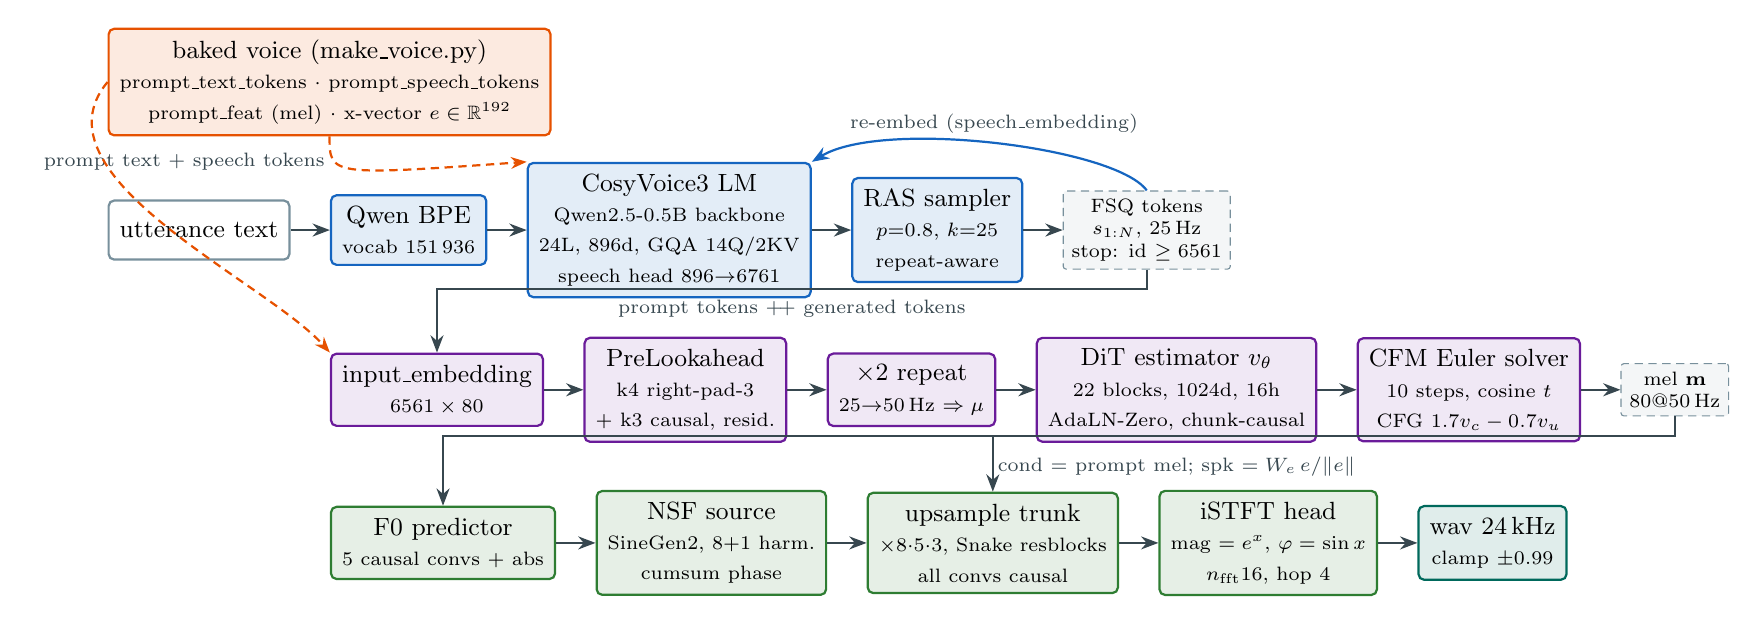
\begin{tikzpicture}[node distance=3.5mm and 5mm, font=\small]
% conditioning column (left)
\node[condblk, align=center] (voice) at (0,0) {baked voice (make\_voice.py)\\
\scriptsize prompt\_text\_tokens $\cdot$ prompt\_speech\_tokens\\
\scriptsize prompt\_feat (mel) $\cdot$ x-vector $e\in\R^{192}$};
% Stage 1: LM
\node[blk, below=8mm of voice.south west, anchor=north west] (text) {utterance text};
\node[lmblk, right=of text] (bpe) {Qwen BPE\\\scriptsize vocab 151\,936};
\node[lmblk, right=of bpe] (lm) {CosyVoice3 LM\\\scriptsize Qwen2.5-0.5B backbone\\\scriptsize 24L, 896d, GQA 14Q/2KV\\\scriptsize speech head 896$\to$6761};
\node[lmblk, right=of lm] (ras) {RAS sampler\\\scriptsize $p{=}0.8$, $k{=}25$\\\scriptsize repeat-aware};
\node[databox, right=of ras] (toks) {FSQ tokens\\\scriptsize $s_{1:N}$, 25\,Hz\\\scriptsize stop: id $\ge 6561$};
\draw[arr] (text) -- (bpe); \draw[arr] (bpe) -- (lm); \draw[arr] (lm) -- (ras);
\draw[arr] (ras) -- (toks);
\draw[arr, cLM] (toks.north) .. controls +(-0.4,0.55) and +(0.9,0.55) .. (lm.north east)
     node[midway, above, lbl]{re-embed (speech\_embedding)};
\draw[condarr] (voice.south) .. controls +(0,-0.5) .. (lm.north west)
     node[pos=0.3, left, lbl]{prompt text $+$ speech tokens};
% Stage 2: flow
\node[flowblk, below=11mm of bpe.south west, anchor=north west] (emb) {input\_embedding\\\scriptsize $6561\times 80$};
\node[flowblk, right=of emb] (pla) {PreLookahead\\\scriptsize k4 right-pad-3\\\scriptsize $+$ k3 causal, resid.};
\node[flowblk, right=of pla] (up) {$\times 2$ repeat\\\scriptsize 25$\to$50\,Hz $\Rightarrow \mu$};
\node[flowblk, right=of up] (dit) {DiT estimator $\vth$\\\scriptsize 22 blocks, 1024d, 16h\\\scriptsize AdaLN-Zero, chunk-causal};
\node[flowblk, right=of dit] (euler) {CFM Euler solver\\\scriptsize 10 steps, cosine $t$\\\scriptsize CFG $1.7v_c - 0.7 v_u$};
\node[databox, right=of euler] (melbox) {mel $\mel$\\\scriptsize $80@50$\,Hz};
\draw[arr] (toks.south) -- ++(0,-2.5mm) -| (emb.north)
     node[pos=0.25, below, lbl]{prompt tokens $+\!+$ generated tokens};
\draw[arr] (emb) -- (pla); \draw[arr] (pla) -- (up); \draw[arr] (up) -- (dit);
\draw[arr] (dit) -- (euler); \draw[arr] (euler) -- (melbox);
\draw[condarr] (voice.west) .. controls +(-1.0,-1.2) and +(-0.8,0.9) .. (emb.north west)
     node[pos=0.8, left, lbl]{};
\node[lbl, below=0.5mm of dit] {\scriptsize cond $=$ prompt mel; spk $= W_e\,e/\lVert e\rVert$};
% Stage 3: vocoder
\node[vocblk, below=10mm of emb.south west, anchor=north west] (f0) {F0 predictor\\\scriptsize 5 causal convs $+$ abs};
\node[vocblk, right=of f0] (nsf) {NSF source\\\scriptsize SineGen2, 8$+$1 harm.\\\scriptsize cumsum phase};
\node[vocblk, right=of nsf] (trunk) {upsample trunk\\\scriptsize $\times8{\cdot}5{\cdot}3$, Snake resblocks\\\scriptsize all convs causal};
\node[vocblk, right=of trunk] (istft) {iSTFT head\\\scriptsize mag $=e^{x}$, $\varphi=\sin x$\\\scriptsize $n_{\mathrm{fft}}16$, hop 4};
\node[audioblk, right=of istft] (wav) {wav 24\,kHz\\\scriptsize clamp $\pm 0.99$};
\draw[arr] (melbox.south) -- ++(0,-2.5mm) -| (f0.north);
\draw[arr] (melbox.south) -- ++(0,-2.5mm) -| (trunk.north);
\draw[arr] (f0) -- (nsf); \draw[arr] (nsf) -- (trunk);
\draw[arr] (trunk) -- (istft); \draw[arr] (istft) -- (wav);
\end{tikzpicture}%
}
\caption{CosyVoice3-0.5B pipeline as ported. Top: the autoregressive LM decodes 25\,Hz
finite-scalar-quantized speech tokens under RAS sampling, conditioned on the baked
voice's prompt transcript and prompt speech tokens; each sampled token is re-embedded
through the speech embedding, not the text embedding. Middle: the conditional
flow-matching stage embeds prompt$+$generated tokens, applies a 3-token lookahead
convolution, upsamples $25\to50$\,Hz to form the semantic conditioning $\mu$, and
integrates a 10-step CFG-guided Euler ODE through a 22-block DiT whose attention is full
offline and chunk-causal when streaming. Bottom: the fully causal HiFT vocoder (NSF
harmonic source $+$ iSTFT head) renders mel to waveform.}
\label{fig:cosy}
\end{figure}

\begin{table}[htbp]
\centering
\caption{CosyVoice3-0.5B exact hyperparameters (frozen port spec; verified against
checkpoint shapes at export).}
\label{tab:cosy-hparams}
\small
\begin{tabular}{@{}llll@{}}
\toprule
\textbf{Stage} & \textbf{Component} & \textbf{Value} & \textbf{Notes} \\
\midrule
Global & sample rate & 24\,000\,Hz & mono fp32 out \\
 & token rate $\ftok$ & 25\,Hz & 1 token $=$ 40\,ms \\
 & mel rate $\fmel$ & 50\,Hz & 1 token $\to$ 2 mel frames; hop 480 \\
 & streaming chunk & 25 tokens & $=$ 50 mel frames $=$ 1\,s audio \\
\midrule
LM & backbone & Qwen2.5-0.5B & hidden states only; own LM head unused \\
 & layers / hidden & 24 / 896 & RMSNorm $\varepsilon{=}10^{-6}$ \\
 & attention & GQA 14Q/2KV, $d_h{=}64$ & q/k/v biased, o\_proj unbiased \\
 & RoPE & $\theta = 10^{6}$, full & all 64 dims rotated \\
 & MLP & 4864, SiLU & gate/up/down \\
 & text vocab & 151\,936 & Qwen BPE; \code{<|endofprompt|>} $=$ 151646 \\
 & speech embedding & $6761 \times 896$ & 6561 FSQ $+$ sos/eos/task/fill $+$ tail \\
 & speech head & Linear $896 \to 6761$ & untied, no bias \\
 & stop rule & id $\ge 6561$ & suppressed below $2\times$ text len; cap $20\times$ \\
\midrule
Flow & token embedding & $6561 \times 80$ & \\
 & lookahead & 3 tokens & conv $k4$ right-pad 3 $+$ $k3$ causal, residual \\
 & speaker proj. & Linear $192 \to 80$ & input L2-normalized x-vector \\
 & DiT & 22 blocks, 1024d, 16h$\times$64 & FF 2048, GELU(tanh), LN affine-free \\
 & AdaLN-Zero & Linear $1024 \to 6144$/block & shift/scale/gate for MSA and MLP \\
 & conv. pos.\ emb. & 2$\times$ ($k31$, groups 16, Mish) & causal (left-pad 30), residual \\
 & time embedding & sinusoidal 256 $\to$ MLP 1024 & scale 1000 \\
 & solver & Euler, 10 steps & $t = 1-\cos(\tau\pi/2)$ \\
 & CFG rate & $w = 0.7$ & $\tilde v = 1.7\,v_c - 0.7\,v_u$ \\
 & noise & fixed $\mathcal{N}$ buffer $[80,15000]$ & seed-0 export; bit-reproducible \\
 & streaming mask & 50-frame chunks & keys $j < (\lfloor i/50\rfloor{+}1)\cdot 50$ \\
 & overlap cache & prompt $+$ last 34 frames & pins the re-solved ODE overlap \\
\midrule
Vocoder & upsampling & $[8,5,3]$, kernels $[16,11,7]$ & nearest $\times s$ then causal conv \\
 & resblocks & $k[3,7,11]$, $d[1,3,5]$, Snake & source resblocks $k[7,7,11]$ \\
 & iSTFT & $n_{\mathrm{fft}}$ 16, hop 4 & mag $=\exp$, phase $=\sin$ direct \\
 & NSF & 8$+$1 harmonics & $A{=}0.1$, $\sigma{=}0.003$, $f_{uv}{=}10$\,Hz \\
 & conv\_pre & $k5$, \emph{right}-causal & 4 mel frames of lookahead \\
 & F0 predictor & 5 causal convs $+$ Linear, ELU & first conv right-pad 3 (lookahead) \\
\bottomrule
\end{tabular}
\end{table}

\subsection{The discrete speech code: finite scalar quantization}
\label{sec:fsq}

The interface between the LM and the acoustic model is a 25\,Hz stream of integers from
a codebook of size $6561 = 3^8$ --- the fingerprint of \emph{finite scalar quantization}
(FSQ). Where classical VQ-VAE learns an explicit codebook and suffers codebook collapse
and commitment-loss tuning, FSQ simply bounds and rounds each dimension of a low-dimensional
latent. A speech encoder (in CosyVoice3, a supervised speech tokenizer distilled from an
ASR encoder; it runs offline, never in the game) produces $z \in \R^{8}$ per 40\,ms
frame; each component is squashed and rounded to $L = 3$ levels:
\begin{equation}
\tilde z_i \;=\; \operatorname{round}\!\big( \tfrac{L-1}{2}\,\tanh(z_i) \big)
\;\in\; \{-1, 0, 1\},
\qquad
\mathrm{id} \;=\; \sum_{i=1}^{8} \big(\tilde z_i + 1\big)\, 3^{\,i-1}
\;\in\; \{0, \dots, 6560\},
\label{eq:fsq}
\end{equation}
with a straight-through estimator through the rounding during tokenizer training. The
implicit codebook is the full product grid $\{-1,0,1\}^8$: every code is used by
construction, the code space is smooth (adjacent ids differ in one scalar level), and
the LM's output distribution over 6561 classes is learnable at 0.5B scale. The token
rate is the single most important constant in the whole system: at 25\,Hz, one second of
speech is 25 classification decisions --- \emph{three orders of magnitude} less than raw
audio-sample autoregression --- which is what makes LM-based TTS decode at real time on a
laptop GPU at all. The 200-row tail above the codebook holds control ids
(\code{sos} 6561, \code{eos} 6562, \code{task\_id} 6563, \code{fill} 6564); every id
$\ge 6561$ terminates decoding, a defensive union that makes any control-id leak a stop
rather than a corrupt flow input.

\subsection{Stage 1: the text-to-token language model}
\label{sec:cosy-lm}

The LM is a stock Qwen2.5-0.5B decoder (24 layers, hidden 896, grouped-query attention
14Q/2KV, full rotary embedding $\theta = 10^6$) with its text head discarded and two
speech-side modules bolted on: a speech embedding ($6761 \times 896$) and an untied
linear speech head ($896 \to 6761$). Reusing a text-pretrained backbone is the family's
quiet superpower --- the model brings text understanding (abbreviations, numbers,
emphasis-bearing punctuation) ``for free'' and needs only learn the text$\to$acoustics
mapping. The inference-time sequence layout is
\begin{equation}
\big[\ \underbrace{\mathrm{sos}}_{\text{speech emb}} \ \big|\
\underbrace{\mathrm{BPE}(\text{prompt text}) \ +\!\!+\ \mathrm{BPE}(\text{utterance
text})}_{\text{text embeddings}} \ \big|\
\underbrace{\mathrm{task\_id}}_{\text{speech emb}} \ \big|\
\underbrace{s^{p}_{1:M}}_{\text{prompt speech tokens}} \ \big],
\label{eq:lm-layout}
\end{equation}
after which autoregressive decoding begins: hidden state $\to$ speech head $\to$
log-softmax $\to$ RAS sampling, and the sampled token is re-embedded \emph{through the
speech embedding} (not the text embedding) for the next step. Layout~\eqref{eq:lm-layout}
is the zero-shot cloning mechanism seen from the LM's side: the prompt transcript and
the prompt's FSQ tokens form an in-context (text, speech) exemplar, and the model
continues the pattern for new text in the same voice --- style transfer as pure
in-context learning, no fine-tuning, no speaker embedding in the LM at all. It also has
a consequential KV-cache implication for games: because the utterance text sits
\emph{between} \code{sos}$+$prompt-text and \code{task\_id}$+$prompt-speech-tokens, only
the $[\mathrm{sos} \mid \text{prompt text}]$ prefix is text-independent and reusable
across utterances of the same voice; the tail must re-prefill every call. (Contrast
Chatterbox, whose layout puts all conditioning first and the text last, making the whole
conditioning prefix cacheable --- a rare point where the older design is
friendlier.)

\subsubsection{RAS sampling: repetition-aware nucleus sampling}
\label{sec:ras}

Speech-token LMs have a characteristic failure mode: local loops (a token or short cycle
repeating), which render as buzzes or stuck vowels. CosyVoice3's sampler counters it
directly. Per step, over the full 6761-way distribution $p$:
\begin{enumerate}[leftmargin=2em]
\item \textbf{Nucleus-with-cap}: sort $p$ descending; keep the smallest prefix with
cumulative mass $< p_{\mathrm{top}} = 0.8$, additionally capped at $k = 25$ candidates;
renormalize and sample a candidate $c$.
\item \textbf{Repetition check}: if $c$ already appeared at least
$\lceil W \tau_r \rceil = 1$ time among the last $W = 10$ emitted tokens, reject it and
resample from the \emph{plain} softmax with $c$ masked out --- deliberately jumping
outside the nucleus to break the loop.
\end{enumerate}
Termination is likewise guarded on both sides: \code{eos} is \emph{suppressed} until at
least $2\times$ the text-token count has been emitted (preventing premature cutoffs on
short prompts --- a 25\,Hz frame rate means roughly 2--20 speech tokens per text token
in practice), and decoding hard-stops at $20\times$ the text length (bounding the damage
of a runaway loop that survives RAS). For parity validation the sampler runs greedy
($k{=}1$); in the game a seed parameter switches between deterministic synthesis (for
reproducible probes) and free randomness.

\subsection{Stage 2: conditional flow matching over mel}
\label{sec:cfm}

The acoustic decoder must turn a token sequence --- which encodes \emph{what} is said
and its coarse prosody, at 25\,Hz --- into an 80-band, 50\,Hz mel spectrogram carrying
the fine acoustic detail the tokens discard. CosyVoice3 does this with \emph{conditional
flow matching} (CFM): a continuous-time generative model that learns a velocity field
transporting Gaussian noise to data.

\subsubsection{Flow matching in brief}

Let $x_1 \sim q(\cdot \mid \mathrm{cond})$ be a data sample (the mel segment) and
$x_0 \sim \mathcal{N}(0, I)$. Define the (optimal-transport / rectified) interpolation
path with a small floor $\sigma_{\min}$:
\begin{equation}
x_t \;=\; \big(1 - (1-\sigma_{\min})\,t\big)\, x_0 \;+\; t\, x_1,
\qquad t \in [0,1],
\label{eq:ot-path}
\end{equation}
whose conditional velocity is constant in $t$:
\begin{equation}
u_t(x_t \mid x_1, x_0) \;=\; \frac{d x_t}{dt} \;=\; x_1 - (1-\sigma_{\min})\, x_0 .
\label{eq:cfm-target}
\end{equation}
Training regresses a network $\vth$ onto this target,
\begin{equation}
\mathcal{L}_{\mathrm{CFM}}(\theta) \;=\;
\E_{t,\,x_0,\,x_1}\;
\big\lVert\, \vth(x_t,\, t;\ \mu,\, c,\, s) \;-\; u_t(x_t \mid x_1, x_0) \,\big\rVert^2 ,
\label{eq:cfm-loss}
\end{equation}
where the conditioning triple is: $\mu$ --- the token-derived semantic track;
$c$ --- a partially known mel ``canvas'' (prompt mel frames filled in, zeros
elsewhere); and $s$ --- the projected speaker vector. With $\sigma_{\min} = 10^{-6}$,
Eq.~\eqref{eq:ot-path} is rectified flow in all but name: straight-line paths, whose
practical payoff is that \emph{few} Euler steps integrate them accurately --- CosyVoice3
uses 10, and distilled relatives (Section~\ref{sec:chatterbox}) reach 1--2.

\subsubsection{Inference: guided Euler on a cosine grid}

At synthesis, sample $x_0$ and integrate $\dot x = \vth(x,t;\cdot)$ from $t=0$ to $1$.
Two refinements matter. First, \emph{classifier-free guidance} (CFG): the estimator is
evaluated with and without conditioning and extrapolated,
\begin{equation}
\tilde v(x, t) \;=\; (1 + w)\, \vth(x, t;\ \mu, c, s)\;-\; w\, \vth(x, t;\ 0, 0, 0),
\qquad w = 0.7,
\label{eq:cfg}
\end{equation}
i.e.\ $\tilde v = 1.7\,v_{\mathrm{cond}} - 0.7\,v_{\mathrm{uncond}}$, sharpening
adherence to the tokens and the voice at the cost of a second estimator evaluation per
step (the two rows run as a batch of 2 --- or should; running them as two separate
passes was one of the port's measured inefficiencies,
Section~\ref{sec:roadmap}). Second, the step grid is \emph{cosine-warped}: with uniform
$\tau_k = k/K$, $K = 10$,
\begin{equation}
t_k \;=\; 1 - \cos\!\Big(\frac{\tau_k\, \pi}{2}\Big), \qquad
x_{k+1} = x_k + (t_{k+1} - t_k)\;\tilde v(x_k, t_k),
\label{eq:euler-cosine}
\end{equation}
which concentrates steps near $t = 0$ (small early steps where the field bends most,
long late steps where rectified paths are nearly straight). Total estimator cost:
$K \times 2 = 20$ DiT forwards per synthesized segment --- the single most expensive
computation in the whole pipeline and the object of most of the optimization work in
Section~\ref{sec:roadmap}.

One further port-specific decision earns a paragraph because it changes the
\emph{semantics} of streaming: the initial noise $x_0$ is not sampled at runtime but
loaded --- a fixed $[80, 15000]$-frame Gaussian buffer exported from the reference
implementation (seed 0) and indexed by absolute frame position. This makes the entire
flow stage \emph{deterministic given the tokens} (bit-reproducible parity with the
Python reference, no RNG-injection hooks in kernels), and, crucially for streaming, it
makes ``the noise at frame $j$'' a well-defined global object independent of chunk
boundaries --- a prerequisite for re-solving a growing prefix and getting identical
early frames (Section~\ref{sec:prefix-stable}).

\subsubsection{From tokens to $\mu$: embedding, lookahead, upsampling}

The semantic track is built causally-with-bounded-lookahead:
\begin{equation}
\mu \;=\; \operatorname{repeat}_{\times 2}\!\Big(
\mathrm{PreLookahead}\big( E[\,s^{p}_{1:M} +\!\!+\, s_{1:N}\,] \big) \Big)
\ \in\ \R^{2(M+N) \times 80},
\label{eq:mu}
\end{equation}
where $E$ is the $6561\times80$ token embedding and \code{PreLookahead} is a $k{=}4$
convolution right-padded by 3 (each position sees exactly 3 \emph{future} tokens)
followed by a causal $k{=}3$ convolution and a residual add. This is the architecture's
explicitly budgeted future context: 3 tokens $=$ 120\,ms. It is a design contract, not
an implementation detail --- the streaming scheduler must hold back exactly 3 tokens
from each chunk boundary so that the lookahead convolution sees real tokens rather than
padding (Section~\ref{sec:schedule}); in exchange, coarticulation across chunk
boundaries is handled by construction rather than by crossfading. The $\times 2$
repeat-interleave takes 25\,Hz tokens to the 50\,Hz mel grid.

\subsubsection{The DiT estimator and the chunk-causal attention mask}
\label{sec:dit}

The estimator $\vth$ is a 22-block diffusion transformer (width 1024, 16 heads of 64,
FF 2048 with tanh-GELU). Its input projection concatenates the four information streams
channel-wise per frame --- state $x_t$, canvas $c$, semantic $\mu$, broadcast speaker
$s$: $[x; c; \mu; s] \in \R^{T\times 320} \to \R^{T\times 1024}$ --- followed by a causal
convolutional position embedding (two $k{=}31$, 16-group convolutions with Mish,
left-padded, residual). Timestep conditioning uses \emph{AdaLN-Zero}: a 256-d sinusoidal
embedding of $t$ (scale 1000) passes through an MLP to 1024, and each block derives
$(\mathrm{shift}, \mathrm{scale}, \mathrm{gate})$ pairs for its attention and MLP
sub-layers from a per-block Linear($1024 \to 6144$) applied to $\mathrm{SiLU}(t_{\mathrm{emb}})$:
\begin{equation}
y = x + g_{\mathrm{msa}} \odot
\mathrm{MHA}\!\big( \mathrm{LN}(x)\,(1 + \sigma_{\mathrm{msa}}) + \delta_{\mathrm{msa}} \big),
\qquad
z = y + g_{\mathrm{mlp}} \odot
\mathrm{FF}\!\big( \mathrm{LN}(y)\,(1 + \sigma_{\mathrm{mlp}}) + \delta_{\mathrm{mlp}} \big),
\label{eq:adaln-zero}
\end{equation}
with affine-free LayerNorms ($\varepsilon = 10^{-6}$) and RoPE ($\theta = 10^4$) applied
to queries and keys. Note what the AdaLN modulations do \emph{not} depend on: the
sequence. They are functions of the timestep alone --- 22 blocks $\times$ 6 vectors
$\times$ 10 timesteps of pure precomputation per synthesis, an observation worth real
milliseconds in the port (Section~\ref{sec:roadmap}). (A port-discovered subtlety for
reproducers: the reference applies RoPE with \emph{interleaved} pair layout
$(2j, 2j{+}1)$ on the \emph{flat} 1024-d vector before head splitting --- with the
consequence that only head 0 is actually rotated. Matching the reference bit-for-bit
means reproducing this faithfully, quirk and all.)

The attention mask is where offline and streaming synthesis diverge --- and
\emph{only} here; weights and everything else are shared:
\begin{equation}
\text{offline:}\quad \mathrm{mask}_{ij} = 1\ \forall i,j
\qquad\qquad
\text{streaming:}\quad \mathrm{mask}_{ij} = 1 \iff
j \;<\; \Big( \big\lfloor i / 50 \big\rfloor + 1 \Big) \cdot 50 ,
\label{eq:chunk-mask}
\end{equation}
i.e.\ frame $i$ attends to every frame of its own 50-frame (1\,s) chunk ---
\emph{including positions after $i$ within the chunk} --- plus all previous chunks, and
never beyond its chunk's right edge. Figure~\ref{fig:chunkmask} visualizes the resulting
block-lower-triangular structure. This \emph{chunk-causal} pattern is the load-bearing
compromise of the whole design: bidirectional context inside a chunk (mel frames need
future context at the tens-of-ms scale for coarticulation), strict causality across
chunks (so a chunk, once rendered, is never invalidated by later tokens). The
model is \emph{trained} with this mask for streaming use, so chunked inference is the
model operating exactly as trained --- not an approximation of an offline model, which
is the fundamental difference from the windowed retrofit of
Section~\ref{sec:chatterbox-stream}.

\begin{figure}[htbp]
\centering
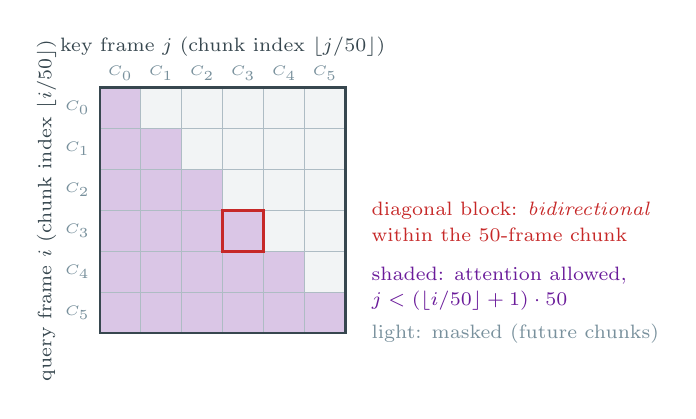
\begin{tikzpicture}[scale=0.52]
% grid of 6x6 chunk blocks; allowed = block-lower-triangular incl diagonal
\foreach \i in {0,...,5} {
  \foreach \j in {0,...,5} {
    \pgfmathparse{\j<=\i ? 1 : 0}
    \ifnum\pgfmathresult>0
      \fill[cFlow!25] (\j, -\i-1) rectangle ++(1,1);
    \else
      \fill[cGrey!10] (\j, -\i-1) rectangle ++(1,1);
    \fi
  }
}
\draw[cGrey!60, step=1] (0,-6) grid (6,0);
\draw[thick, cText] (0,-6) rectangle (6,0);
% chunk labels
\foreach \j in {0,...,5} {
  \node[tick] at (\j+0.5, 0.35) {$C_{\j}$};
  \node[tick] at (-0.55, -\j-0.5) {$C_{\j}$};
}
\node[lbl, rotate=90] at (-1.3,-3) {query frame $i$ (chunk index $\lfloor i/50\rfloor$)};
\node[lbl] at (3, 1.0) {key frame $j$ (chunk index $\lfloor j/50\rfloor$)};
% annotate one diagonal block
\draw[cWarn, very thick] (3,-4) rectangle (4,-3);
\node[lbl, text=cWarn, anchor=west] at (6.4,-3.0) {diagonal block: \emph{bidirectional}};
\node[lbl, text=cWarn, anchor=west] at (6.4,-3.6) {within the 50-frame chunk};
\node[lbl, text=cFlow, anchor=west] at (6.4,-4.6) {shaded: attention allowed,};
\node[lbl, text=cFlow, anchor=west] at (6.4,-5.2) {$j < (\lfloor i/50\rfloor + 1)\cdot 50$};
\node[lbl, text=cGrey, anchor=west] at (6.4,-6.0) {light: masked (future chunks)};
\end{tikzpicture}
\caption{The chunk-causal attention mask of Eq.~\eqref{eq:chunk-mask}, drawn at
chunk granularity ($C_k$ $=$ mel frames $[50k, 50k{+}50)$, i.e.\ 1\,s of audio). Within a
chunk attention is fully bidirectional (fine acoustic context); across chunks it is
strictly causal (streaming safety). Offline synthesis replaces the whole mask with
all-ones --- same weights, one full-attention pass.}
\label{fig:chunkmask}
\end{figure}

\subsubsection{Zero-shot voice conditioning in the flow}

The flow receives the voice through three channels, all precomputed offline by a
voice-baking script (\code{make\_voice.py}) and shipped as data: (i) the prompt's FSQ
tokens are prepended to the generated tokens in Eq.~\eqref{eq:mu}, so $\mu$ begins with
the reference utterance's semantic track; (ii) the prompt's \emph{mel} occupies the
canvas: $c_{1:P} = \mathrm{prompt\ mel}$, $c_{P+1:T} = 0$ --- an inpainting formulation
in which the model literally continues a partially painted spectrogram, anchoring
timbre, channel characteristics, and recording ambience; (iii) a 192-d x-vector from an
external speaker-verification model, L2-normalized and projected to 80-d, is added as a
global bias. The solver integrates the \emph{whole} canvas (prompt rows included) and
discards the first $P$ rows of the result. Baking voices offline keeps the runtime lean
--- the game never runs the speech tokenizer, mel extractor, or x-vector network; a
voice is four tensors in the weights manifest. The same mechanism yields cross-family
reuse: the shipped \code{velmire} voice was baked from a reference clip synthesized by
\emph{Kokoro} (voice \code{am\_onyx}) --- one TTS cloning another's speaker identity,
which collapses voice-asset production to ``pick any clean 24\,kHz clip.''

\subsection{Stage 3: the causal HiFT vocoder}
\label{sec:hift}

The final stage maps mel ($80@50$\,Hz) to waveform at 24\,kHz --- an upsampling factor
of 480 $=$ $8 \cdot 5 \cdot 3 \cdot 4$ (three learned stages and the iSTFT hop). The
generator is a HiFT: HiFi-GAN-style trunk, NSF excitation, iSTFT head --- the same
science as Kokoro's generator (Section~\ref{sec:kokoro-gen}) with one systematic
difference that defines it: \emph{every convolution is causal}, in the padding-discipline
sense. Standard ``same'' padding splits $(k-1)$ zeros symmetrically, so every layer
leaks $\lfloor (k{-}1)/2 \rfloor$ frames of future; stacked over $\sim$20 layers and
three upsamplings, an offline HiFT's receptive field reaches hundreds of ms into the
future --- which is exactly why offline vocoders produce edge garbage when truncated at
a chunk boundary (measured quantitatively in Section~\ref{sec:chatterbox-stream}). The
causal variant instead pads each convolution entirely on one side:
left (past) by default; \emph{right} (future) only in two audited places that
constitute the vocoder's explicit lookahead budget --- the mel-input convolution
(\code{conv\_pre}, $k{=}5$, 4 mel frames $=$ 80\,ms of future) and the F0 predictor's
first convolution (3 frames). During streaming, non-final chunks simply withhold those
few tail frames (rendering them next chunk when their right context exists), and all
per-convolution state (the left-pad contents), the NSF's running phase, and the iSTFT
overlap-add tail are carried across chunks. Upsampling is nearest-neighbor followed by a
causal convolution rather than transposed convolution --- same expressive role, no
future taps, no checkerboarding. The head predicts 9 log-magnitudes and 9 phase angles
($n_{\mathrm{fft}} = 16$, hop 4; phase read directly as $\varphi = \sin(x)$, no atan2 in
the graph), and the F0 predictor is a 5-conv causal stack with ELU and $|\cdot|$ output
--- no recurrence despite its reference name, though the reference runs it in float64
and the port gates its fp32 GPU version against a drift-sensitive parity dump.

\subsection{Shared vocoder science: the neural source-filter model}
\label{sec:nsf}

Both vocoders (and Chatterbox's) share the NSF excitation principle, which deserves its
own statement since it is the reason neural vocoders stopped producing pitch artifacts.
GAN vocoders that generate waveform purely from mel must \emph{infer} phase and
periodicity; NSF instead computes the periodic part analytically from the predicted F0
and lets the network shape it. With $f_0[n]$ the frame-rate pitch track upsampled to
sample rate, harmonic index $h \in \{1, \dots, H{+}1\}$ ($H = 8$ overtones plus the
fundamental):
\begin{equation}
\phi_h[n] \;=\; 2\pi \Big( \sum_{m \le n} \frac{h\, f_0[m]}{\fs} \Big) \bmod 2\pi
\;+\; \phi_h^{(0)},
\qquad
e_h[n] \;=\; A \sin \phi_h[n],
\label{eq:nsf-phase}
\end{equation}
a cumulative-sum phase so that pitch changes glide without discontinuities
($\phi_h^{(0)}$ random initial phases; $A = 0.1$). A voicing gate mixes harmonics with
noise:
\begin{equation}
u[n] = \mathbf{1}\{f_0[n] > f_{uv}\}, \qquad
s[n] = \tanh\!\Big( W \big[\, u\, e_{1:H+1} + \sigma_n \varepsilon \,\big] \Big),
\qquad \varepsilon \sim \mathcal{N}(0, I),
\label{eq:nsf-mix}
\end{equation}
with $f_{uv} = 10$\,Hz, $\sigma_n$ small in voiced regions and larger ($A/3$) in
unvoiced ones, and $W$ a learned $(H{+}1) \to 1$ mix. The source $s[n]$ enters the
generator trunk at multiple scales through small conv adapters (in CausalHiFT, via an
STFT of the source, downsampled by strided causal convs to each trunk resolution), and
the trunk acts as the learned \emph{filter} of a classical source-filter decomposition:
harmonic structure guaranteed by construction, spectral envelope and aperiodicity
learned. Two real-time-relevant engineering notes: the cumulative sum in
Eq.~\eqref{eq:nsf-phase} reaches $10^4$--$10^5$ radians over long utterances, so the
phase accumulator must be fp32 even in an otherwise fp16 pipeline (measured failure mode:
fp16 phase turns sustained vowels metallic); and in streaming the accumulator is
\emph{carried state} --- restarting phase per chunk is instantly audible as a click,
which is one of the quantified lessons of the Chatterbox windowing study
(Section~\ref{sec:chatterbox-stream}).

\subsection{Why the AR token architecture is real-time-native}
\label{sec:why-ar}

Assembling the pieces: every stage of Family~B exposes a commit point at or below one
second of audio, by construction rather than by approximation ---
\begin{itemize}[leftmargin=2em]
\item the \textbf{LM} is causal token-by-token; its KV cache carries the full acoustic
history (prompt and everything spoken so far) into every new token at $O(1)$
incremental cost;
\item the \textbf{flow} is chunk-causal with a trained mask
(Eq.~\ref{eq:chunk-mask}) and a 3-token bounded lookahead (Eq.~\ref{eq:mu}); a chunk's
mel depends only on tokens up to its right edge plus 3;
\item the \textbf{vocoder} is causal with an audited 4-mel-frame lookahead and carried
conv/phase/OLA state.
\end{itemize}
Prosodic coherence follows from the same structure that yields streamability: chunk
$k$'s mel is generated \emph{conditioned on all previous chunks} --- through the LM's
autoregressive state, through the flow's cross-chunk attention to the entire mel
prefix, and through the vocoder's carried state --- so pitch declination, rhythm, and
phrasal structure continue across chunk boundaries instead of resetting as in the
clause-chunked non-AR pipeline (Section~\ref{sec:kokoro-noar}). The cost side of the
ledger is equally structural: a sampling loop that must be rate-guarded
(Section~\ref{sec:ras}), $20$ DiT forwards per segment, and --- in the current port ---
a re-solve-the-prefix streaming implementation whose per-chunk cost grows with utterance
length (the measured consequence and its remedy are quantified in
Sections~\ref{sec:schedule} and~\ref{sec:roadmap}). The next section examines what
happens when this causality discipline is absent and streaming must be imposed from
outside.

% ============================================================================
\section{Family C: Chatterbox-Turbo, the offline-designed contrast}
\label{sec:chatterbox}
% ============================================================================

Chatterbox-Turbo is the instructive control experiment: an AR token front end
(so Stage~1 streams exactly like CosyVoice3's) attached to an acoustic decoder designed
without streaming in mind. Studying why it \emph{cannot} emit mid-utterance --- and what
happened when the project tried to force it to --- sharpens the claims of
Section~\ref{sec:why-ar} into measured facts.

\subsection{Architecture}

The token LM (``T3'') is a GPT2-medium backbone --- 24 layers, hidden 1024, 16-head MHA,
learned absolute position embeddings, biased projections throughout --- with text and
speech embeddings and an untied speech head over a 6563-way speech vocabulary
(6561 codes $+$ start/stop). Conditioning is a prefix of one projected 256-d speaker
embedding plus 375 reference speech tokens; then text tokens; then AR speech decoding
with conventional HF-style sampling (temperature 0.8, top-$k$ 1000, top-$p$ 0.95,
repetition penalty 1.2). Note the contrast with RAS: repetition \emph{penalty} reshapes
logits globally and permanently, while RAS \emph{rejects} locally --- the latter
preserves the model's calibrated distribution except at the moment of a detected loop.

The acoustic decoder (``S3Gen'') converts tokens to mel with a flow model in the same
mathematical family as Section~\ref{sec:cfm} --- but distilled for few-step inference
(the turbo release runs \emph{2} solver steps) and, decisively, \emph{bidirectional}: a
conformer-style token encoder and a flow estimator that attend over the whole utterance
with no chunk mask and no trained streaming mode. The vocoder is a standard
(non-causal) HiFT. On paper this buys quality per parameter: full right context
everywhere, and a 2-step solver that made Chatterbox the \emph{fastest} acoustic stage
of the three ports per mel frame. Measured end-to-end $\RTF = 1.42$ on the RTX~4060 ---
between Kokoro and CosyVoice3 --- yet it is the \emph{least} real-time-capable system of
the three, because none of that compute can begin until the LM has finished the entire
utterance, and none of the audio can be released until the whole flow solve completes.
\TTFA{} is therefore bounded below by full-utterance token decode plus full-utterance
flow --- for a 10\,s line, several seconds regardless of optimization.

\subsection{Retrofitting streams: clause pipelining and the windowed-flow study}
\label{sec:chatterbox-stream}

The shipped mitigation is the same one non-AR systems use: cut text into clauses, run
the full offline pipeline per clause, pipeline synthesis against playback through the
ring buffer (Section~\ref{sec:composition}). This works --- Chatterbox voiced the
project's NPC demo for months --- but inherits both non-AR drawbacks (\TTFA{} $=$
first-clause latency; prosody resets per clause) \emph{plus} keeps the AR sampling loop's
cost and failure modes: the worst of both families, redeemed by output quality.

More interesting for this document is the project's controlled attempt at \emph{true}
streaming --- windowing the flow over 1\,s token windows while T3 was still decoding ---
because its failure modes were quantified before the effort was superseded by
CosyVoice3's trained-for-streaming design. Three findings, from a seeded A/B probe
harness (fixed sampled token sequence; windowed variants differ from the offline render
only in windowing):

\begin{enumerate}[leftmargin=2em]
\item \textbf{Vocoder edge contamination is severe but exactly repairable.} The final
frames of any truncated HiFT render are convolution/iSTFT edge garbage. Measured
artifact-to-signal profile as a function of distance from a cut edge: $-2$\,dB at 0
frames, $-15$\,dB at 4, $-44$\,dB at 8, $-59$\,dB at 16 (20\,ms frames); left edges
similar ($-45$\,dB at 8). Keeping edge-touching samples was the dominant audible defect
--- seam noise 3--5\,dB \emph{louder} than the speech in the 40--100\,ms before every
seam. The repair is purely geometric: render $[s{-}C_M,\, e{+}R_M]$, emit $[s, e)$, with
$C_M = 32$ frames of left context and $R_M = 16$ frames of right render margin, plus a
10\,ms equal-power crossfade of two renders of the same instant at each seam. After
this, the worst 20\,ms bin of (windowed $-$ offline) measured $-40$\,dB --- inaudible.
The general lesson: \emph{non-causal vocoders can be streamed by overprovisioning
context}, at a fixed latency cost ($R_M = 320$\,ms here) and redundant compute.
\item \textbf{NSF phase must be global.} Restarting the harmonic phase accumulator
(Eq.~\ref{eq:nsf-phase}) per window produces an audible discontinuity at every seam;
the fix is generating the source globally (or carrying cumulative phase as streaming
state) and slicing per window. This lesson transferred directly into the CausalHiFT
port's carried-state design (Section~\ref{sec:hift}).
\item \textbf{The flow itself resists windowing.} A window re-rendered fresh from noise
continues \emph{its own} realization of the utterance, not the one already emitted ---
diffusion-family models sample a distribution, and two solves with different context
windows land on audibly different ``takes,'' producing take-switch seams. Teacher
forcing the already-emitted mel into the estimator's canvas channel (the same inpainting
pathway used for the voice prompt) mostly repairs continuity --- this is, in fact,
CosyVoice's own chunked-flow mechanism rediscovered --- but a residual onset artifact
at the first seam survived every window/context/lookahead configuration tried
($W{=}25$ tokens, $C{=}50$ context, 5 lookahead), with the windowed \emph{encoder}
(token context truncation, i.e.\ precisely the absence of a trained chunk-causal
attention) as the prime suspect when the effort was paused.
\end{enumerate}

The synthesis of the study is the central negative result of this document:
\emph{everything about offline flow TTS can be streamed by brute force except the
acoustic model's context handling --- which is exactly the part CosyVoice3 fixes by
training with the chunk mask of Eq.~\eqref{eq:chunk-mask}}. Streaming is an
architecture-and-training property, not a deployment trick.

% ============================================================================
\section{Streaming schedules for AR token TTS}
\label{sec:streaming}
% ============================================================================

This section specifies the token-level streaming machinery of the CosyVoice3 port
exactly --- schedule, masking, state, and the end-to-end timeline --- since it is the
concrete realization of the ``real-time-native'' claim.

\subsection{The chunk schedule: 25 $\to$ 50 $\to$ 100 with 3-token lookahead}
\label{sec:schedule}

The LM decodes continuously in a single pass (one prefill, then one token per step,
KV-cached). Interleaved with decoding, the scheduler watches the count of
not-yet-rendered tokens and fires an acoustic chunk when a hop's worth plus the
lookahead is available. Three refinements make the schedule exact
(Figure~\ref{fig:schedule}):

\begin{enumerate}[leftmargin=2em]
\item \textbf{Prompt-alignment padding.} The flow's chunk grid
(Eq.~\ref{eq:chunk-mask}) counts \emph{mel frames from the start of the canvas},
which begins with the $M$ prompt tokens. The first hop is therefore enlarged by
$\mathrm{pad} = \lceil M / 25 \rceil \cdot 25 - M$ tokens so that prompt $+$ first hop
lands exactly on a 50-mel-frame chunk boundary; all later chunk edges then stay
grid-aligned automatically.
\item \textbf{Hop doubling.} The hop starts at 25 tokens (1\,s) and doubles after each
emitted chunk, capped at 100: $25 \to 50 \to 100 \to 100 \to \cdots$. Early chunks are
small to minimize \TTFA{}; later chunks are large to amortize per-chunk overhead
(each chunk re-enters the flow solver, so fewer, larger chunks cost less total compute)
--- by the time the third chunk fires, the ring buffer holds seconds of margin and
latency no longer matters.
\item \textbf{Lookahead holdback.} A chunk covering tokens $[o, o{+}h)$ is rendered
only once $o + h + 3$ tokens exist, and the 3 extras enter the flow as
\code{PreLookahead} context only --- they are not part of the emitted rows and are
re-rendered as owned tokens in the next chunk. The \textbf{finalize} chunk (fired at
EOS) releases the holdback: everything renders, the vocoder's lookahead tails are not
trimmed, and carried state is flushed.
\end{enumerate}

\begin{figure}[htbp]
\centering
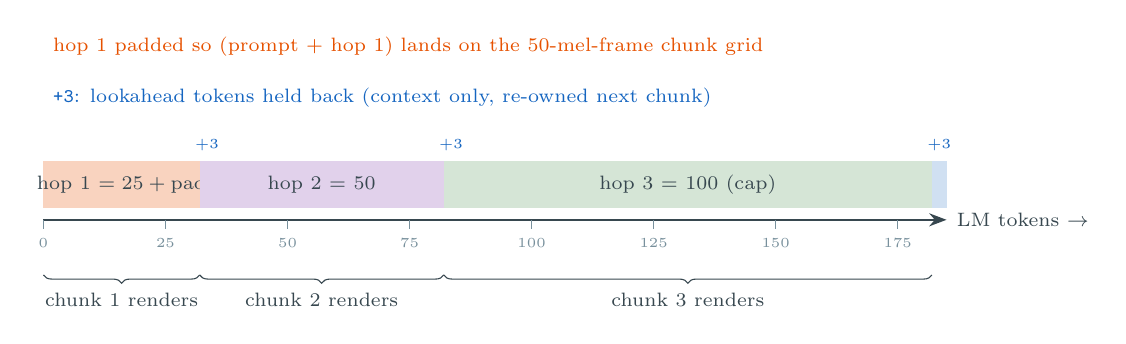
\begin{tikzpicture}[xscale=0.062, font=\small]
% token axis 0..180
\draw[arr] (0,0) -- (185,0) node[right, lbl] {LM tokens $\to$};
\foreach \x in {0,25,...,175} \draw[cGrey] (\x,0) -- (\x,-0.12) node[below, tick] {\x};
% prompt pad segment (first hop enlarged): assume pad = 7 for illustration
\fill[cCond!25] (0,0.15) rectangle (32,0.75);
\node[lbl] at (16,0.45) {hop 1 $= 25 + \mathrm{pad}$};
\fill[cLM!20] (32,0.15) rectangle (35,0.75);
\node[tick, text=cLM] at (33.5,0.95) {$+3$};
% chunk 2: hop 50
\fill[cFlow!20] (32,0.15) rectangle (82,0.75);
\node[lbl] at (57,0.45) {hop 2 $=$ 50};
\fill[cLM!20] (82,0.15) rectangle (85,0.75);
\node[tick, text=cLM] at (83.5,0.95) {$+3$};
% chunk 3: hop 100
\fill[cVoc!20] (82,0.15) rectangle (182,0.75);
\node[lbl] at (132,0.45) {hop 3 $=$ 100 (cap)};
\fill[cLM!20] (182,0.15) rectangle (185,0.75);
\node[tick, text=cLM] at (183.5,0.95) {$+3$};
% emitted audio rows
\draw[decorate, decoration={brace, amplitude=3pt, mirror}, cText] (0,-0.7) -- (32,-0.7)
  node[midway, below=3pt, lbl] {chunk 1 renders};
\draw[decorate, decoration={brace, amplitude=3pt, mirror}, cText] (32,-0.7) -- (82,-0.7)
  node[midway, below=3pt, lbl] {chunk 2 renders};
\draw[decorate, decoration={brace, amplitude=3pt, mirror}, cText] (82,-0.7) -- (182,-0.7)
  node[midway, below=3pt, lbl] {chunk 3 renders};
\node[lbl, anchor=west, text=cCond] at (0,2.2)
  {hop 1 padded so (prompt $+$ hop 1) lands on the 50-mel-frame chunk grid};
\node[lbl, anchor=west, text=cLM] at (0,1.55)
  {\code{+3}: lookahead tokens held back (context only, re-owned next chunk)};
\end{tikzpicture}
\caption{The CosyVoice3 streaming chunk schedule on the token axis. Hops double
$25 \to 50 \to 100$ (capped), the first hop absorbs the prompt-alignment pad, and every
non-final chunk waits for 3 extra lookahead tokens that feed the \code{PreLookahead}
convolution but are not emitted. Each fired chunk renders 1--4\,s of new audio.}
\label{fig:schedule}
\end{figure}

\subsection{Prefix stability: earlier frames are bit-identical}
\label{sec:prefix-stable}

The current implementation re-solves the flow over the whole growing prefix each chunk
(then re-runs the vocoder over the full generated mel, emitting only samples past the
already-played offset). This sounds wasteful --- it is, quantifiably, and
Section~\ref{sec:roadmap} addresses it --- but it is \emph{correct} in a strong sense:
because (i) the noise buffer is indexed by absolute frame (Section~\ref{sec:cfm}),
(ii) the chunk mask forbids any frame from attending beyond its chunk's right edge, and
(iii) the token prefix is append-only, frame $i$'s entire computation in chunk $k$ is
input-identical to its computation in chunk $k{+}1$. Already-emitted audio is therefore
\emph{bit-identical} across re-solves --- verified in the port's stream probe, and
additionally cross-checked against the offline path (the streaming and offline renders
agree exactly on every completed chunk; only the final partial chunk differs by the
untrimmed lookahead). An overlap cache (prompt frames plus the last 34 mel frames of
the previous chunk, pinned as $(z, \mu)$ state) exists in the reference design for the
incremental variant, where it guarantees the re-solved ODE agrees on the seam region.
Prefix stability is what makes the ring buffer contract trivial: samples, once pushed,
are never revised, so the audio thread needs no notion of retraction --- the property
that the windowed-Chatterbox study (Section~\ref{sec:chatterbox-stream}) spent margin
frames and crossfades approximating is here exact by construction.

\subsection{The end-to-end timeline and the latency budget}
\label{sec:timeline}

Figure~\ref{fig:timeline} assembles the whole streaming path on a wall-clock axis, and
Figure~\ref{fig:latency-stack} decomposes the measured \TTFA{}. Reading
Eq.~\eqref{eq:ttfa-decomp} against measured stage rates on the RTX~4060: the first
chunk needs $N_1 = 25 + \mathrm{pad} + 3$ tokens ($\approx$\,28--50 depending on the
voice's prompt length); at 49.8 tokens/s the token wait is 0.6--1.0\,s; the first flow
chunk solves a short sequence (prompt $+$ 50 frames) through $10\times2$ DiT forwards;
the first vocoder chunk is comparatively negligible (vocoder-stage $\RTF \approx
0.34$); and readback, ring prebuffer, and frame-slicing stretch fill the remainder of
the measured $\TTFA = 4.65$\,s (fp16, pre-optimization). The decomposition identifies
the flow as the dominant term and the token wait as the irreducible floor
($\approx$\,1.1\,s of audio must exist as tokens before anything can render --- the
price of the 25-token chunk, which is itself the price of the trained chunk grid).

\begin{figure}[htbp]
\centering
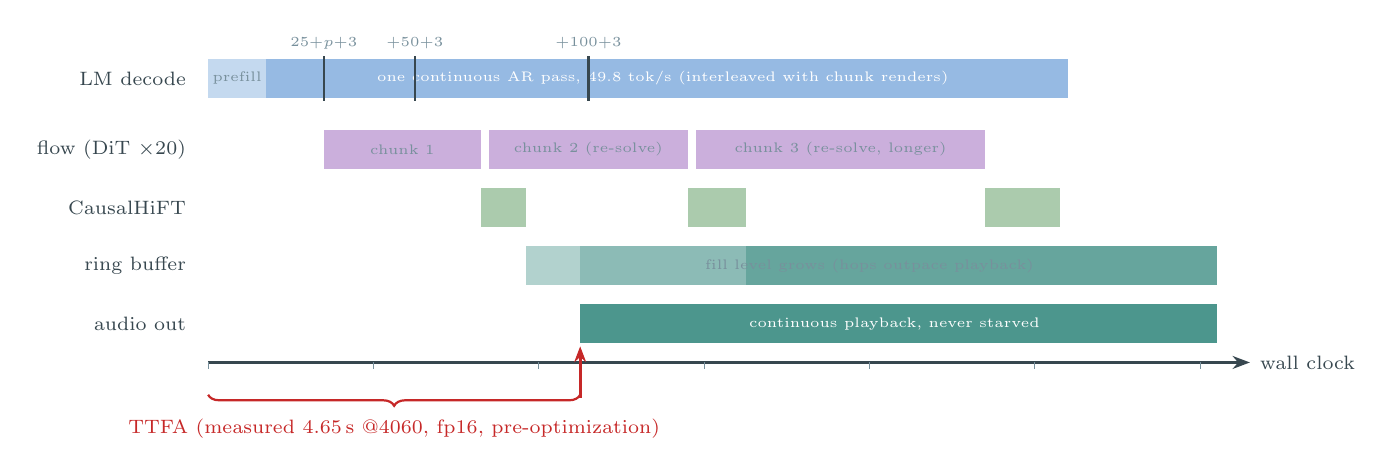
\begin{tikzpicture}[xscale=1.05, yscale=0.82, font=\small]
% time axis
\draw[arr] (0,0) -- (12.6,0) node[right, lbl] {wall clock};
\foreach \x/\l in {0/0, 2/{}, 4/{}, 6/{}, 8/{}, 10/{}, 12/{}}
  \draw[cGrey] (\x,0) -- (\x,-0.1);
% Row 5: LM decode
\node[lbl, anchor=east] at (-0.15,4.4) {LM decode};
\fill[cLM!25] (0,4.1) rectangle (0.7,4.7);
\node[tick] at (0.35,4.4) {prefill};
\fill[cLM!45] (0.7,4.1) rectangle (10.4,4.7);
\node[tick, text=white] at (5.5,4.4) {one continuous AR pass, 49.8 tok/s (interleaved with chunk renders)};
\foreach \x in {1.4, 2.5, 4.6} \draw[cText, thick] (\x,4.05) -- (\x,4.75);
\node[tick] at (1.4,4.95) {$25{+}p{+}3$};
\node[tick] at (2.5,4.95) {$+50{+}3$};
\node[tick] at (4.6,4.95) {$+100{+}3$};
% Row 4: flow solves
\node[lbl, anchor=east] at (-0.15,3.3) {flow (DiT $\times$20)};
\fill[cFlow!35] (1.4,3.0) rectangle (3.3,3.6);   \node[tick] at (2.35,3.3) {chunk 1};
\fill[cFlow!35] (3.4,3.0) rectangle (5.8,3.6);   \node[tick] at (4.6,3.3) {chunk 2 (re-solve)};
\fill[cFlow!35] (5.9,3.0) rectangle (9.4,3.6);   \node[tick] at (7.65,3.3) {chunk 3 (re-solve, longer)};
% Row 3: vocoder
\node[lbl, anchor=east] at (-0.15,2.4) {CausalHiFT};
\fill[cVoc!40] (3.3,2.1) rectangle (3.85,2.7);
\fill[cVoc!40] (5.8,2.1) rectangle (6.5,2.7);
\fill[cVoc!40] (9.4,2.1) rectangle (10.3,2.7);
% Row 2: ring buffer
\node[lbl, anchor=east] at (-0.15,1.5) {ring buffer};
\fill[cAudio!30] (3.85,1.2) rectangle (4.5,1.8);
\fill[cAudio!45] (4.5,1.2) rectangle (6.5,1.8);
\fill[cAudio!60] (6.5,1.2) rectangle (12.2,1.8);
\node[tick] at (8.0,1.5) {fill level grows (hops outpace playback)};
% Row 1: audio out
\node[lbl, anchor=east] at (-0.15,0.6) {audio out};
\fill[cAudio!70] (4.5,0.3) rectangle (12.2,0.9);
\node[tick, text=white] at (8.3,0.6) {continuous playback, never starved};
% TTFA marker
\draw[cWarn, very thick, -{Stealth[length=2mm]}] (4.5,-0.55) -- (4.5,0.25);
\draw[cWarn, thick, decorate, decoration={brace, amplitude=4pt, mirror}] (0,-0.5) -- (4.5,-0.5)
  node[midway, below=5pt, lbl, text=cWarn] {$\TTFA$ (measured 4.65\,s @4060, fp16, pre-optimization)};
\end{tikzpicture}
\caption{Streaming timeline (schematic, proportions from measured stage rates). The LM
decodes once, continuously; chunk renders (flow $+$ vocoder) fire at the schedule of
Fig.~\ref{fig:schedule} and interleave with further decoding on the same GPU; new
samples land in the ring buffer, and playback starts once the prebuffer threshold is
met, defining \TTFA{}. Hop doubling makes each later chunk deliver more audio per fire,
so the ring's fill level --- the starvation margin --- grows over the utterance.}
\label{fig:timeline}
\end{figure}

\begin{figure}[htbp]
\centering
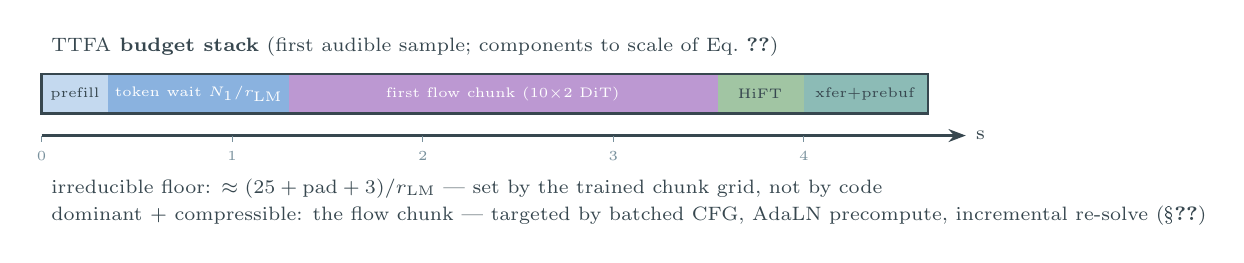
\begin{tikzpicture}[xscale=2.42, font=\small]
\node[lbl, anchor=west] at (0, 0.85) {\textbf{\TTFA{} budget stack} (first audible sample; components to scale of Eq.~\ref{eq:ttfa-decomp})};
% stacked bar, total ~4.65 (units: seconds)
\fill[cLM!25]  (0,0)    rectangle (0.35,0.5);
\fill[cLM!50]  (0.35,0) rectangle (1.30,0.5);
\fill[cFlow!45](1.30,0) rectangle (3.55,0.5);
\fill[cVoc!45] (3.55,0) rectangle (4.00,0.5);
\fill[cAudio!45](4.00,0) rectangle (4.65,0.5);
\draw[cText, thick] (0,0) rectangle (4.65,0.5);
\node[tick, text=cText] at (0.175,0.25) {prefill};
\node[tick, text=white] at (0.825,0.25) {token wait $N_1/r_{\mathrm{LM}}$};
\node[tick, text=white] at (2.42,0.25) {first flow chunk (10$\times$2 DiT)};
\node[tick, text=cText] at (3.77,0.25) {HiFT};
\node[tick, text=cText] at (4.32,0.25) {xfer$+$prebuf};
% axis
\draw[arr] (0,-0.28) -- (4.85,-0.28) node[right, lbl] {s};
\foreach \x in {0,1,...,4} \draw[cGrey] (\x,-0.28) -- (\x,-0.36) node[below, tick] {\x};
% annotations
\node[lbl, anchor=west] at (0,-0.95) {irreducible floor: $\approx (25 + \mathrm{pad} + 3)/r_{\mathrm{LM}}$ --- set by the trained chunk grid, not by code};
\node[lbl, anchor=west] at (0,-1.3) {dominant + compressible: the flow chunk --- targeted by batched CFG, AdaLN precompute, incremental re-solve (\S\ref{sec:roadmap})};
\end{tikzpicture}
\caption{Decomposition of the measured 4.65\,s \TTFA{} on the RTX~4060 (fp16 CosyVoice3,
schematic proportions). The token wait is an architectural floor; the flow solve is the
engineering target.}
\label{fig:latency-stack}
\end{figure}

\subsection{Token-level vs.\ clause-level streaming, and text--audio sync UX}
\label{sec:sync-ux}

The two streaming granularities now on the table are not competitors so much as tiers
with different couplings to the dialogue LLM:

\begin{itemize}[leftmargin=2em]
\item \textbf{Clause-level} (Kokoro, Chatterbox): text enters per clause; audio exits
per clause. \TTFA{} $=$ first-clause synthesis; prosody resets per clause;
implementation is simple (each clause is an independent offline job against a shared
ring). Because synthesis input is textual, the system composes naturally with a
\emph{still-decoding} LLM: speech of clause 1 plays while the LLM writes clause 3.
\item \textbf{Token-level} (CosyVoice3): text enters per clause/utterance (the
non-bistream LM conditions on complete text --- Eq.~\ref{eq:lm-layout}); audio exits
per second. \TTFA{} decouples from utterance length; prosody is coherent across the
whole utterance. The residual coupling --- needing the full utterance text before
speech-token decoding starts --- can be hidden behind the LLM's own decode time in
practice (the utterance is complete before the previous one finishes playing), and the
reference architecture's ``bistream'' mode (interleaving text and speech tokens in one
sequence, with a \code{fill} control token when speech outruns text) removes it
entirely at the cost of a more delicate schedule; the port deliberately defers it.
\end{itemize}

Either way, a game needs one more piece of machinery that pure-TTS treatments omit:
\textbf{text--audio synchronization for the UI}. Players read subtitles; an NPC whose
transcript appears seconds before (or after) the voice reads as broken. The transport
layer solves this with sample-counter bookkeeping rather than heuristics: the ring
buffer maintains monotonic counters of samples written and read; when a clause is
queued for synthesis, its future start position is recorded as the current
written-count; a per-frame pump fires a reveal event the moment the read-counter
(i.e.\ actual playback position) crosses a clause's start minus a configurable lead
(0.35\,s in the shipped \code{KokoroVoice}, so text leads voice slightly, matching
subtitle convention). Talk animations key off a separate predicate --- ``ring playing
and non-empty'' --- rather than ``synthesis in progress,'' so mouths do not flap during
synthesis stalls. These details are cheap, but only exist because the transport owns
exact sample-position truth; a design that hands the audio system opaque clips per
clause has to reconstruct them heuristically.

% ============================================================================
\section{GPU inference inside a game engine}
\label{sec:engine}
% ============================================================================

Everything so far treated the models as if they ran on a benign server. This section
treats the deployment reality that constitutes the dissertation's novel contribution:
all three TTS families (plus the dialogue LLMs and two STT models) run \emph{inside
Unity}, entirely on the GPU, with no ML runtime whatsoever --- no ONNX Runtime, no
Sentis, no native plugins, no Python. A shipped game contains C\# code, \code{.compute}
shaders (HLSL), and exported weight binaries. The motivations are control and
portability: a runtime framework imposes its own scheduling (fatal for frame-budget
discipline, Section~\ref{sec:slicing}), its own memory management (fatal for latent
loading, Section~\ref{sec:latent}), and a dependency surface; hand-written kernels make
every dispatch, byte, and synchronization point visible and budgetable.

\subsection{Architecture of the runtime}
\label{sec:runtime-arch}

The runtime is organized as a strict class hierarchy --- \code{ModelBase} $\to$ family
bases (\code{LLM}/\code{TTS}/\code{STT}) $\to$ concrete models --- so that residency,
budgets, and warmup are uniform across every model in the pool. Conventions that carry
architectural weight:

\begin{itemize}[leftmargin=2em]
\item \textbf{Weights} are exported offline by a Python exporter into per-tensor
\code{.bin} files plus a \code{manifest.tsv} (name, file, dtype, element count, shape).
The manifest is the schema: the exporter tracks consumed checkpoint keys and fails on
leftovers, so a completed export is provably complete. fp16 tensors pack two values per
32-bit word; int8 tensors pack four, with a per-row scale sidecar
(Section~\ref{sec:int8}). Norms, embeddings, and heads always stay fp16; embedding
tables are sharded ($\times$16) so no single upload step exceeds the frame budget.
\item \textbf{Kernels}: one \code{.compute} file per model family, uniform
bind-and-dispatch idiom, every shader registered in a lazy central registry. Weight-norm
reparameterizations are folded at export ($w = g\,v / \lVert v \rVert$), biases fused
where the reference had them, and activation quirks (tanh-GELU vs.\ erf-GELU, LeakyReLU
slopes, $(1{+}\gamma)$ norms) implemented exactly --- the parity harness
(Section~\ref{sec:parity}) exists precisely because such details are where ports die.
\item \textbf{GPU-only runtime with audited exceptions}: models never ship a CPU
inference backend; CPU twins exist strictly as validation oracles. The sole exception is
microsecond-scale \emph{sequential} cells where per-step GPU dispatch overhead would
dominate compute by orders of magnitude: Kokoro's six biLSTMs (hidden 256/direction,
$\le$1500 steps, $\sim$10\,MFLOP per pass --- microseconds on CPU, but thousands of
serial dispatches on GPU) run as flat C\# loops inside the GPU pipeline, a documented
hybrid boundary per model rather than a fallback path. This is the small-scale mirror
of the dispatch-bound analysis of Section~\ref{sec:int8}.
\end{itemize}

\subsection{Frame discipline: coroutines and MAC-budget slicing}
\label{sec:slicing}

Unity's main loop is single-threaded around the render loop; the mechanism for
long-running work is the \emph{coroutine} --- a resumable iterator that yields control
back to the engine and continues next frame. Every stage of every model in the runtime
is a coroutine: weight upload yields under a bytes-per-frame budget, kernel warmup
compiles one shader variant per frame behind the loading screen, LM decoding yields per
token (or per layer during prefill), and --- the interesting case --- dense synthesis
stages yield under a \emph{MAC budget}.

The problem the MAC budget solves: a Kokoro clause synthesis is a few hundred kernel
dispatches totaling tens of GFLOPs. Dispatched in one frame, that is a multi-frame
freeze (Section~\ref{sec:framebudget}); dispatched one kernel per frame, synthesis takes
seconds of wall-clock and the ring starves. The right granularity is \emph{work},
not \emph{kernels}: the pipeline accumulates an analytic estimate of multiply-accumulate
operations issued since the last yield and yields when it crosses a threshold:
\begin{equation}
\mathrm{acc} \mathrel{+}= \widehat{\mathrm{MAC}}(\mathrm{dispatch});
\qquad
\mathrm{acc} \ge B_{\mathrm{MAC}} \;\Rightarrow\; \big(\ \mathrm{yield};\
\mathrm{acc} \leftarrow 0\ \big),
\qquad B_{\mathrm{MAC}} = 2.5\times 10^{8},
\label{eq:macslice}
\end{equation}
where each dispatch site contributes its closed-form cost (e.g.\ $3\,C_{\mathrm{in}}
C_{\mathrm{out}} T$ for a $k{=}3$ convolution over $T$ frames, $2\,T^2 d + T d^2$ for an
attention layer). $B_{\mathrm{MAC}} = 2.5\times10^8$ MACs corresponds to roughly
2--3\,ms of GPU work on the RTX~4060 --- a slice that coexists with a 30\,FPS render
load. The estimates need only be \emph{proportional}, not exact: the budget is a
scheduling knob, and a single scalar recalibrates it per hardware tier.

The measured outcome on the shipped Kokoro$+$Qwen NPC stack: with an LLM feeding text
deltas and Kokoro synthesizing and playing concurrently, the \emph{speak-alone}
scenario drops 2 frames in 5544 above the 33\,ms line --- effectively hitch-free
speech synthesis on a mid-range laptop GPU while the game renders. The residual spikes
in the combined scenario (38 frames in 1267 during LLM decode) were traced not to
synthesis but to the LLM's per-token \emph{synchronous logits readback} --- a
GPU$\to$CPU stall, not compute --- with the remedy (async readback one token behind,
trading a token of latency for zero stalls) on the roadmap. The
diagnosis generalizes into a rule: \emph{in frame-budgeted inference, synchronization
points --- not FLOPs --- are the first thing to profile.}

\subsection{Latent loading: budgeted weight streaming tied to gameplay}
\label{sec:latent}

A 1--2\,GB weight set cannot load during gameplay with a blocking call (seconds-long
freeze), and should not necessarily be resident at all times (VRAM is shared with the
renderer and \emph{other models} --- the NPC stack co-resides an LLM, a TTS, and
eventually an STT). The runtime therefore treats GPU residency as a first-class,
gameplay-visible state machine on \code{ModelBase}
(Figure~\ref{fig:residency}):

\begin{itemize}[leftmargin=2em]
\item \code{Prefetch()} begins streaming weights under a per-instance
\emph{bytes-per-frame} budget sampled every frame --- upload proceeds only in
frame-affordable slices. \code{SlowPrefetch(seconds)} solves the budget from a target
duration: given bytes remaining and a time goal, stream so residency completes just in
time. \code{BoostFetch()} raises the budget when stealth no longer matters (loading
screen, cutscene); \code{PausePrefetch()} suspends without discarding progress.
\item \code{Defetch(Full|Slow)} releases GPU residency --- immediately, or budgeted
frame-by-frame in reverse. In-flight IO is \emph{epoch-invalidated}: a Defetch during a
load races nothing (stale completions are discarded by epoch check), and a Prefetch
issued during a Defetch is queued, never lost.
\item The gameplay binding is spatial: NPCs carry a \emph{prefetch zone} (a 10\,m
trigger sphere in the shipped demo). Player enters $\to$ \code{SlowPrefetch} sized to
approach time (weights arrive as the player walks up); player leaves $\to$ budgeted
defetch. The design philosophy --- \emph{heavy work hides where the player is not
looking} --- also governs kernel prewarming (one throwaway micro-synthesis compiles all
shader paths behind the zone boundary, so the first real line has no compile hitch) and
extends to LLM-side background work (conversation compaction between dialogue turns).
\end{itemize}

\begin{figure}[htbp]
\centering
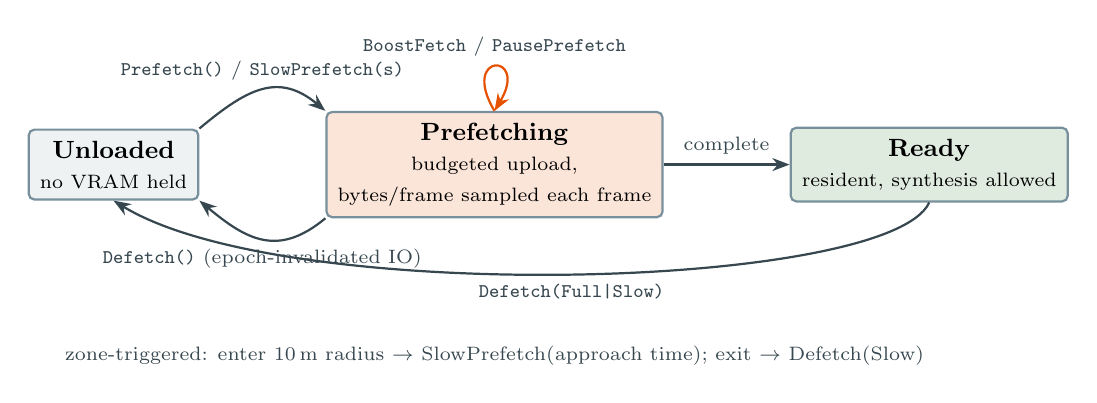
\begin{tikzpicture}[node distance=9mm and 16mm, font=\small]
\node[blk, fill=cGrey!12] (unloaded) {\textbf{Unloaded}\\\scriptsize no VRAM held};
\node[blk, fill=cCond!15, right=of unloaded] (prefetching) {\textbf{Prefetching}\\\scriptsize budgeted upload,\\\scriptsize bytes/frame sampled each frame};
\node[blk, fill=cVoc!15, right=of prefetching] (ready) {\textbf{Ready}\\\scriptsize resident, synthesis allowed};
\draw[arr] (unloaded.north east) .. controls +(0.6,0.5) and +(-0.6,0.5) .. (prefetching.north west)
  node[midway, above, lbl] {\code{Prefetch()} / \code{SlowPrefetch(s)}};
\draw[arr] (prefetching) -- (ready) node[midway, above, lbl] {complete};
\draw[arr] (prefetching.south west) .. controls +(-0.6,-0.5) and +(0.6,-0.5) .. (unloaded.south east)
  node[midway, below, lbl] {\code{Defetch()} (epoch-invalidated IO)};
\draw[arr] (ready.south) .. controls +(-0.5,-1.1) and +(2.2,-1.35) .. (unloaded.south)
  node[pos=0.5, below, lbl] {\code{Defetch(Full|Slow)}};
\draw[arr, cCond] (prefetching.north) .. controls +(-0.45,0.75) and +(0.45,0.75) .. (prefetching.north)
  node[midway, above, lbl] {\code{BoostFetch} / \code{PausePrefetch}};
\node[lbl, below=15mm of prefetching] {zone-triggered: enter 10\,m radius $\to$ SlowPrefetch(approach time); exit $\to$ Defetch(Slow)};
\end{tikzpicture}
\caption{The residency lifecycle on \code{ModelBase} (``latent loading''). All
transitions are anti-frame-drop: uploads and releases proceed in per-frame byte budgets,
mid-load cancellation is race-free via epoch-invalidated IO, and a prefetch issued
during an in-progress defetch is queued rather than lost.}
\label{fig:residency}
\end{figure}

\subsection{int8 quantization: memory-bound vs.\ dispatch-bound}
\label{sec:int8}

The runtime's quantization scheme is deliberately simple: symmetric per-row int8 on
matmul weights only,
\begin{equation}
W_{r,:} \;\approx\; s_r\, q_{r,:}, \qquad
s_r = \frac{\max_j |W_{r,j}|}{127}, \qquad
q_{r,j} = \operatorname{round}\!\big( W_{r,j} / s_r \big) \in [-127, 127],
\label{eq:int8}
\end{equation}
packed four per 32-bit word with an fp16 scale sidecar; activations remain fp32/fp16,
dequantization happens in-register in the matmul kernel, and norms, embeddings, and
heads stay fp16. Accuracy is a non-issue at this scheme's granularity for these models:
Kokoro int8 (78 quantized matmuls) shows max weight-reconstruction error $\le 0.011$
with no audible change; CosyVoice3 int8 holds LM log-probability correlation 0.999867
and flow-mel correlation 0.9996 against fp32. (A methodological aside: int8 waveform
outputs decorrelate against the reference \emph{waveform} despite excellent mel
correlation --- tiny mel perturbations shift vocoder phase, and sample-domain
correlation collapses under phase drift while the audio is perceptually identical. The
correct int8 acceptance gate is the \emph{mel}, the last pre-phase representation. Gate
placement is part of methodology design, Section~\ref{sec:parity}.)

The performance result is the instructive part. The naive expectation --- ``half the
bytes, twice the speed for memory-bound stages'' --- collides with measurement:

\begin{itemize}[leftmargin=2em]
\item \textbf{LM decode: dispatch-overhead-bound, int8 gains nothing.} Single-token
decode is a chain of small GEMVs: arithmetically memory-bound in the textbook sense,
but each kernel is so small ($\sim$microseconds of math) that per-dispatch fixed cost
--- command submission, binding, barriers --- dominates. The CosyVoice3 LM issues
$\approx$240 dispatches per generated token; measured decode is 51.6 tokens/s at int8
vs.\ 49.8 at fp16 --- a 3.6\% difference. Halving the bytes did nothing because bytes
were not the bottleneck; the roadmap remedy is \emph{dispatch fusion} (fewer, larger
kernels per layer), not lower precision.
\item \textbf{Flow: compute-bound after tiling, int8 gains nothing.} The optimized DiT
runs coalesced tiled fp16 GEMMs at batch $T{=}$ hundreds of frames; measured flow time
is 6.9\,s vs.\ 7.0\,s (int8 vs.\ fp16) at $T{=}576$ --- ALU-saturated, so weight
bandwidth is again not the limiter. End-to-end streaming $\RTF$: 2.90 (int8) vs.\ 2.86
(fp16) --- statistically flat.
\item \textbf{What int8 does buy: residency.} CosyVoice3 drops from 1.9\,GB to
996\,MB; Kokoro to 143\,MB. On an 8\,GB card shared with a renderer and an LLM, halving
the TTS footprint is the difference between co-residency and thrashing --- and it also
halves \emph{prefetch time} at a fixed bytes-per-frame budget, a real gameplay latency
(the latent-loading path of Section~\ref{sec:latent} streams half the bytes).
\end{itemize}

The general law extracted: \emph{quantization accelerates only the regime where weight
bytes are the binding constraint --- large-batch, well-fused, memory-bound kernels. In
small-model on-device inference, the binding constraint is often dispatch overhead or
ALU throughput, and the durable wins of int8 are VRAM footprint and load time.} Deciding
where a stage sits requires measuring it; both intuitions (``GEMV is memory-bound'',
``GEMM is compute-bound'') were only half-right until profiled in situ.

% ============================================================================
\section{Measured results and validation methodology}
\label{sec:results}
% ============================================================================

\subsection{The parity harness}
\label{sec:parity}

Porting a neural network across frameworks, languages, \emph{and} numerical precision
without a correctness oracle is hopeless; the project's methodology makes the oracle
explicit and per-stage. For each model:

\begin{enumerate}[leftmargin=2em]
\item A Python \code{dump\_reference.py} runs the original implementation and saves
every stage boundary as \code{.npy}: for CosyVoice3 --- text tokens, step-0 LM logits,
the sampled token sequence (greedy for determinism), the flow's post-lookahead hidden,
the 50\,Hz $\mu$, the step-0 DiT input and cond/uncond velocities, the final mel; the
vocoder's F0 track, NSF source, and waveform.
\item \textbf{All stochasticity is exported as data.} Sampling runs greedy; the flow's
initial noise is the fixed seed-0 buffer shipped \emph{as a weight}
(Section~\ref{sec:cfm}); NSF noise and initial phases are dumped and injected. The
Unity render is then a deterministic function of the same inputs --- ``noise as
weights'' turns a statistical comparison into an exact one.
\item The Unity probe loads the dumps, runs its pipeline stage by stage, and gates each
boundary on Pearson correlation, threshold 0.99. In practice the shipped ports sit far
above the gate: Kokoro passes all 26 kernels and every stage at corr $= 1.000000$;
CosyVoice3's stages measure 1.000000 (LM hidden states through all 24 layers, flow
lookahead/velocity/mel, vocoder stages) with end-to-end waveform 0.99975--0.999989;
step-0 LM log-probabilities 0.999998 with argmax match.
\item Probes run under a headless batch runner (exit code $+$ completion marker file
--- guarding against a stuck editor process masquerading as success), producing a
machine-readable report per run; listening QA is a separate, final gate.
\end{enumerate}

Two methodological lessons generalize. First, \emph{per-stage gating localizes}: a
wav-level mismatch implicates everything; a mel-level pass with wav-level failure
implicates exactly the vocoder. Second, \emph{gate placement must respect the
representation's stability}: sample-domain correlation is meaningless under phase drift
(the int8 finding of Section~\ref{sec:int8}), so quantized variants gate on mel while
fp16 ports gate on waveform.

\subsection{Results}
\label{sec:results-table}

Table~\ref{tab:results} consolidates the measured numbers; all on an RTX~4060 laptop
GPU inside Unity unless noted.

\begin{table}[htbp]
\centering
\caption{Measured results of the DeepUnity TTS ports (RTX~4060 laptop GPU, in-engine).
$\RTF$ per Eq.~\eqref{eq:rtf}: synthesis wall-clock over audio duration, lower is
better, $< 1$ is real-time. Correlations are Unity-vs-PyTorch parity values
(Section~\ref{sec:parity}).}
\label{tab:results}
\small
\begin{tabular}{@{}llll@{}}
\toprule
\textbf{Quantity} & \textbf{Kokoro-82M} & \textbf{CosyVoice3-0.5B} & \textbf{Chatterbox-Turbo} \\
\midrule
$\RTF$ offline & \textbf{0.24--0.43} & $\approx 2.0$ & 1.42 \\
$\RTF$ streaming & (clause-pipelined) & 2.86 fp16 / 2.90 int8 & (clause-pipelined) \\
\TTFA{} & first-clause synth & 4.65\,s & first-clause synth \\
LM decode rate & --- (non-AR) & 49.8 tok/s ($2.0\times$ RT need) & --- \\
Flow stage & --- & 7.0\,s @ $T{=}576$ (from 23\,s naive) & 2-step solver \\
Vocoder stage $\RTF$ & (in totals) & $\approx$0.34 & (in totals) \\
Weights fp16 & $\approx$164\,MB & 1.9\,GB & --- \\
Weights int8 & 143\,MB & 996\,MB & --- \\
int8 quality & max err $\le$ 0.011 & LM logp 0.999867, mel 0.9996 & --- \\
Parity (stages) & corr 1.000000 (26/26 kernels) & corr 1.000000 all stages & parity PASS \\
Parity (wav) & corr 1.000000 & 0.99975--0.999989 & 0.999 \\
Frame health & speak-alone: 2/5544 $>$ 33\,ms & (pending play-QA) & --- \\
\bottomrule
\end{tabular}
\end{table}

Notable derived observations. (i) Kokoro's $\RTF$ spread (0.24--0.43) tracks utterance
length --- fixed per-chunk overheads amortize better over long clauses. (ii) The
CosyVoice3 optimization pass that took the flow from 23\,s to 7.0\,s at $T = 576$
(coalesced tiled GEMMs, cooperative AdaLN reductions, cached kernel/buffer handles) was
pure kernel engineering with zero model change --- a $3.3\times$ reminder that naive
correct kernels and fast kernels are different artifacts. (iii) Streaming $\RTF$
(2.86) currently \emph{exceeds} offline ($\approx$2.0) because each chunk re-solves the
growing prefix (Section~\ref{sec:prefix-stable}): correctness-first, speed-second was
the porting order, and the gap is the target of the roadmap below.

\subsection{The optimization roadmap: from 2.9 to real time}
\label{sec:roadmap}

The remaining path to $\RTF < 1$ for CosyVoice3 on mid-range hardware is structural
rather than exploratory --- each item attacks a measured, named inefficiency:

\begin{enumerate}[leftmargin=2em]
\item \textbf{Batched CFG} --- run the conditioned and unconditioned estimator rows of
Eq.~\eqref{eq:cfg} as one batch-2 pass instead of two sequential passes: near-halving
of flow wall-clock at fixed FLOPs (better occupancy, half the dispatches).
\item \textbf{AdaLN precompute} --- the DiT's modulation vectors depend only on the
timestep (Section~\ref{sec:dit}): precompute all $22 \times 10$ blocks once per
synthesis; removes $22 \times 10 \times 2$ small matmuls and their dispatch overhead
from the inner loop.
\item \textbf{Incremental chunk re-solve} --- stop re-solving the prefix: freeze
previous chunks' DiT key/value tensors (they cannot change --- the mask guarantees it,
Eq.~\ref{eq:chunk-mask}) and solve only the new chunk's 50--200 frames against cached
context, with the vocoder re-rendering only its short left-context margin. Converts
per-chunk flow cost from $O(T_{\mathrm{prefix}})$ to $O(\mathrm{chunk})$ --- the
streaming analogue of a KV cache, and the item that changes the asymptotics rather
than the constants.
\item \textbf{LM dispatch fusion $+$ async token readback} --- collapse the
$\approx$240 dispatches per token (Section~\ref{sec:int8}) and remove the synchronous
logits readback identified in the frame-health probe (Section~\ref{sec:slicing}).
\end{enumerate}

Items 1--2 are local and low-risk; item 3 rests on the prefix-stability invariant
already validated bit-exact (Section~\ref{sec:prefix-stable}). The combination targets
the flow term of Figure~\ref{fig:latency-stack} --- the dominant, compressible term ---
while the token-wait floor ($\approx$0.6--1.0\,s) remains, by design, the price of the
trained chunk grid.

% ============================================================================
\section{Design guidance and conclusions}
\label{sec:conclusions}
% ============================================================================

\subsection{A model-tier strategy for shipped games}

No single architecture wins all deployment tiers; the measured numbers argue for an
explicit two-tier strategy, selectable per device (and even per NPC):

\begin{itemize}[leftmargin=2em]
\item \textbf{Baseline tier --- non-AR small model (Kokoro-class).} $\RTF \approx 0.3$
leaves a $3\times$ frame-slicing margin (Section~\ref{sec:framebudget}) even on GPUs
several tiers below the RTX~4060; 143\,MB int8 residency co-exists with anything;
determinism means no sampling failure modes to guard in QA. Costs: fixed voicepack
identities and per-clause prosody resets. For ambient NPC chatter, this tier is simply
correct engineering.
\item \textbf{Premium tier --- AR token model (CosyVoice3-class), gated on measured
$\RTF < 1$.} Utterance-coherent prosody, zero-shot voices (including bootstrapping
voices from the baseline tier's output --- the \code{velmire} pattern), token-level
\TTFA{} independent of utterance length. The gate must be \emph{measured on device},
not assumed: until the roadmap of Section~\ref{sec:roadmap} lands the streaming
$\RTF < 1$ on the target tier, the AR model belongs in latency-tolerant contexts
(scripted cutscenes rendered a scene early, or offline bake of semi-dynamic lines).
\item The two tiers compose: same \code{TTS} base class, same ring-buffer transport,
same clause-feeding interface, same residency machinery --- an NPC's voice tier is a
constructor argument, and a mid-session downgrade (thermal throttling, VRAM pressure)
is a defetch$+$prefetch away.
\end{itemize}

\subsection{Findings}

\begin{enumerate}[leftmargin=2em]
\item \textbf{Streaming granularity is an architectural property, fixed at training
time.} Non-AR pipelines are chunk-atomic for three independent structural reasons
(up-front durations, whole-chunk normalization statistics, bidirectional context);
offline flow decoders cannot be windowed into true streaming without seam artifacts
traceable to untrained context truncation; the AR token pipeline streams exactly
because every stage was built and \emph{trained} causal or chunk-causal. Deployment
cannot add what training omitted (Sections~\ref{sec:kokoro-noar},
\ref{sec:chatterbox-stream}, \ref{sec:why-ar}).
\item \textbf{The real-time-native design has a specific, small vocabulary of
mechanisms}, each doing one job: a low-rate discrete code (25\,Hz FSQ) making the LM
loop affordable; bounded lookahead (3 tokens; 4 mel frames) making coarticulation local;
a trained chunk-causal mask making prefixes immutable; fixed absolute-position noise
making chunked stochastic generation coherent; carried vocoder state (conv pads, NSF
phase, OLA tails) making waveform seams exact. Together they yield the streaming
contract a game audio system wants: \emph{samples, once emitted, are final ---
bit-identical to the offline render}.
\item \textbf{In-engine inference is a scheduling problem wearing a modeling costume.}
The differences between a demo and a shippable system were: MAC-budget slicing
(2 dropped frames per 5544), budgeted proximity-triggered weight residency,
prewarming hidden behind gameplay, and profiling that distinguishes memory-bound from
dispatch-bound from ALU-bound stages before reaching for quantization. int8 halved
footprints and load times but bought zero throughput on either the dispatch-bound LM
or the compute-bound flow --- a result that contradicts the default mental model and
was only obtainable by measurement (Section~\ref{sec:int8}).
\item \textbf{Bit-exact parity methodology is what makes any of this tractable.}
Freezing stochasticity as data and gating every stage boundary turns a
cross-framework, cross-precision, cross-language port into a sequence of local,
falsifiable claims --- and the same harness then doubles as the acceptance gate for
quantization and for streaming-vs-offline equivalence (Section~\ref{sec:parity}).
\end{enumerate}

\subsection{Outlook}

Three threads continue past this document. First, completing the CosyVoice3 roadmap
(Section~\ref{sec:roadmap}) to bring trained-causal streaming under $\RTF = 1$ on
mid-range hardware --- at which point the premium tier stops being conditional.
Second, tightening the text-side coupling: the bistream LM variant (interleaved
text/speech tokens) would let speech-token decoding start before the dialogue LLM
finishes a sentence, removing the last per-utterance serialization; type-ahead prefill
of the player's draft input attacks the symmetric latency on the LLM side. Third, the
transport layer's sample-counter design (Section~\ref{sec:sync-ux}) generalizes
beyond subtitles --- viseme streams for lip sync and gesture cues are the same
machinery with different payloads, and a chunk-level emotion re-prompt (swapping the
flow's prompt canvas mid-utterance at a chunk boundary) is an open, architecturally
plausible extension that only a chunk-causal design could even attempt.

The one-sentence summary of the whole document: \emph{for real-time synthetic speech,
choose the architecture whose causality structure matches your streaming contract, and
spend your engineering on the scheduler --- the model was never the only system in the
frame.}

% ============================================================================
\section*{Acknowledgment of sources}
% ============================================================================
\addcontentsline{toc}{section}{Acknowledgment of sources}

All architectural constants, implementation details, and measured figures in this
document derive from the DeepUnity InferenceEngine project artifacts: the frozen port
specifications (\code{TTS/CosyVoice/SPEC.md}, \code{TTS/Kokoro/SPEC.md},
\code{TTS/SPEC.md} for Chatterbox), the subsystem architecture log
(\code{InferenceEngine/CLAUDE.md}), the streaming experiment log
(\code{TTS/STREAMING\_EXPERIMENTS.md}), and the streaming implementations
(\code{CosyVoiceTTS.cs}, \code{KokoroVoice.cs}). The underlying model releases are
Kokoro-82M (hexgrad, Apache-2.0), Fun-CosyVoice3-0.5B (FunAudioLLM), and
Chatterbox-Turbo (Resemble AI); the architectural lineages trace to StyleTTS~2,
FastSpeech~2, ISTFTNet, HiFi-GAN, the neural source-filter model, VALL-E-style codec
LMs, flow matching / rectified flow, classifier-free guidance, finite scalar
quantization, and diffusion transformers with AdaLN-Zero conditioning --- formal
citations to be inserted in the dissertation's bibliography pass.

\end{document}
